\documentclass[11pt]{article}

    \usepackage[breakable]{tcolorbox}
    \usepackage{parskip} % Stop auto-indenting (to mimic markdown behaviour)
    
    \usepackage{iftex}
    \ifPDFTeX
    	\usepackage[T1]{fontenc}
    	\usepackage{mathpazo}
    \else
    	\usepackage{fontspec}
    \fi

    % Basic figure setup, for now with no caption control since it's done
    % automatically by Pandoc (which extracts ![](path) syntax from Markdown).
    \usepackage{graphicx}
    % Maintain compatibility with old templates. Remove in nbconvert 6.0
    \let\Oldincludegraphics\includegraphics
    % Ensure that by default, figures have no caption (until we provide a
    % proper Figure object with a Caption API and a way to capture that
    % in the conversion process - todo).
    \usepackage{caption}
    \DeclareCaptionFormat{nocaption}{}
    \captionsetup{format=nocaption,aboveskip=0pt,belowskip=0pt}

    \usepackage{float}
    \floatplacement{figure}{H} % forces figures to be placed at the correct location
    \usepackage{xcolor} % Allow colors to be defined
    \usepackage{enumerate} % Needed for markdown enumerations to work
    \usepackage{geometry} % Used to adjust the document margins
    \usepackage{amsmath} % Equations
    \usepackage{amssymb} % Equations
    \usepackage{textcomp} % defines textquotesingle
    % Hack from http://tex.stackexchange.com/a/47451/13684:
    \AtBeginDocument{%
        \def\PYZsq{\textquotesingle}% Upright quotes in Pygmentized code
    }
    \usepackage{upquote} % Upright quotes for verbatim code
    \usepackage{eurosym} % defines \euro
    \usepackage[mathletters]{ucs} % Extended unicode (utf-8) support
    \usepackage{fancyvrb} % verbatim replacement that allows latex
    \usepackage{grffile} % extends the file name processing of package graphics 
                         % to support a larger range
    \makeatletter % fix for old versions of grffile with XeLaTeX
    \@ifpackagelater{grffile}{2019/11/01}
    {
      % Do nothing on new versions
    }
    {
      \def\Gread@@xetex#1{%
        \IfFileExists{"\Gin@base".bb}%
        {\Gread@eps{\Gin@base.bb}}%
        {\Gread@@xetex@aux#1}%
      }
    }
    \makeatother
    \usepackage[Export]{adjustbox} % Used to constrain images to a maximum size
    \adjustboxset{max size={0.9\linewidth}{0.9\paperheight}}

    % The hyperref package gives us a pdf with properly built
    % internal navigation ('pdf bookmarks' for the table of contents,
    % internal cross-reference links, web links for URLs, etc.)
    \usepackage{hyperref}
    % The default LaTeX title has an obnoxious amount of whitespace. By default,
    % titling removes some of it. It also provides customization options.
    \usepackage{titling}
    \usepackage{longtable} % longtable support required by pandoc >1.10
    \usepackage{booktabs}  % table support for pandoc > 1.12.2
    \usepackage[inline]{enumitem} % IRkernel/repr support (it uses the enumerate* environment)
    \usepackage[normalem]{ulem} % ulem is needed to support strikethroughs (\sout)
                                % normalem makes italics be italics, not underlines
    \usepackage{mathrsfs}
    

    
    % Colors for the hyperref package
    \definecolor{urlcolor}{rgb}{0,.145,.698}
    \definecolor{linkcolor}{rgb}{.71,0.21,0.01}
    \definecolor{citecolor}{rgb}{.12,.54,.11}

    % ANSI colors
    \definecolor{ansi-black}{HTML}{3E424D}
    \definecolor{ansi-black-intense}{HTML}{282C36}
    \definecolor{ansi-red}{HTML}{E75C58}
    \definecolor{ansi-red-intense}{HTML}{B22B31}
    \definecolor{ansi-green}{HTML}{00A250}
    \definecolor{ansi-green-intense}{HTML}{007427}
    \definecolor{ansi-yellow}{HTML}{DDB62B}
    \definecolor{ansi-yellow-intense}{HTML}{B27D12}
    \definecolor{ansi-blue}{HTML}{208FFB}
    \definecolor{ansi-blue-intense}{HTML}{0065CA}
    \definecolor{ansi-magenta}{HTML}{D160C4}
    \definecolor{ansi-magenta-intense}{HTML}{A03196}
    \definecolor{ansi-cyan}{HTML}{60C6C8}
    \definecolor{ansi-cyan-intense}{HTML}{258F8F}
    \definecolor{ansi-white}{HTML}{C5C1B4}
    \definecolor{ansi-white-intense}{HTML}{A1A6B2}
    \definecolor{ansi-default-inverse-fg}{HTML}{FFFFFF}
    \definecolor{ansi-default-inverse-bg}{HTML}{000000}

    % common color for the border for error outputs.
    \definecolor{outerrorbackground}{HTML}{FFDFDF}

    % commands and environments needed by pandoc snippets
    % extracted from the output of `pandoc -s`
    \providecommand{\tightlist}{%
      \setlength{\itemsep}{0pt}\setlength{\parskip}{0pt}}
    \DefineVerbatimEnvironment{Highlighting}{Verbatim}{commandchars=\\\{\}}
    % Add ',fontsize=\small' for more characters per line
    \newenvironment{Shaded}{}{}
    \newcommand{\KeywordTok}[1]{\textcolor[rgb]{0.00,0.44,0.13}{\textbf{{#1}}}}
    \newcommand{\DataTypeTok}[1]{\textcolor[rgb]{0.56,0.13,0.00}{{#1}}}
    \newcommand{\DecValTok}[1]{\textcolor[rgb]{0.25,0.63,0.44}{{#1}}}
    \newcommand{\BaseNTok}[1]{\textcolor[rgb]{0.25,0.63,0.44}{{#1}}}
    \newcommand{\FloatTok}[1]{\textcolor[rgb]{0.25,0.63,0.44}{{#1}}}
    \newcommand{\CharTok}[1]{\textcolor[rgb]{0.25,0.44,0.63}{{#1}}}
    \newcommand{\StringTok}[1]{\textcolor[rgb]{0.25,0.44,0.63}{{#1}}}
    \newcommand{\CommentTok}[1]{\textcolor[rgb]{0.38,0.63,0.69}{\textit{{#1}}}}
    \newcommand{\OtherTok}[1]{\textcolor[rgb]{0.00,0.44,0.13}{{#1}}}
    \newcommand{\AlertTok}[1]{\textcolor[rgb]{1.00,0.00,0.00}{\textbf{{#1}}}}
    \newcommand{\FunctionTok}[1]{\textcolor[rgb]{0.02,0.16,0.49}{{#1}}}
    \newcommand{\RegionMarkerTok}[1]{{#1}}
    \newcommand{\ErrorTok}[1]{\textcolor[rgb]{1.00,0.00,0.00}{\textbf{{#1}}}}
    \newcommand{\NormalTok}[1]{{#1}}
    
    % Additional commands for more recent versions of Pandoc
    \newcommand{\ConstantTok}[1]{\textcolor[rgb]{0.53,0.00,0.00}{{#1}}}
    \newcommand{\SpecialCharTok}[1]{\textcolor[rgb]{0.25,0.44,0.63}{{#1}}}
    \newcommand{\VerbatimStringTok}[1]{\textcolor[rgb]{0.25,0.44,0.63}{{#1}}}
    \newcommand{\SpecialStringTok}[1]{\textcolor[rgb]{0.73,0.40,0.53}{{#1}}}
    \newcommand{\ImportTok}[1]{{#1}}
    \newcommand{\DocumentationTok}[1]{\textcolor[rgb]{0.73,0.13,0.13}{\textit{{#1}}}}
    \newcommand{\AnnotationTok}[1]{\textcolor[rgb]{0.38,0.63,0.69}{\textbf{\textit{{#1}}}}}
    \newcommand{\CommentVarTok}[1]{\textcolor[rgb]{0.38,0.63,0.69}{\textbf{\textit{{#1}}}}}
    \newcommand{\VariableTok}[1]{\textcolor[rgb]{0.10,0.09,0.49}{{#1}}}
    \newcommand{\ControlFlowTok}[1]{\textcolor[rgb]{0.00,0.44,0.13}{\textbf{{#1}}}}
    \newcommand{\OperatorTok}[1]{\textcolor[rgb]{0.40,0.40,0.40}{{#1}}}
    \newcommand{\BuiltInTok}[1]{{#1}}
    \newcommand{\ExtensionTok}[1]{{#1}}
    \newcommand{\PreprocessorTok}[1]{\textcolor[rgb]{0.74,0.48,0.00}{{#1}}}
    \newcommand{\AttributeTok}[1]{\textcolor[rgb]{0.49,0.56,0.16}{{#1}}}
    \newcommand{\InformationTok}[1]{\textcolor[rgb]{0.38,0.63,0.69}{\textbf{\textit{{#1}}}}}
    \newcommand{\WarningTok}[1]{\textcolor[rgb]{0.38,0.63,0.69}{\textbf{\textit{{#1}}}}}
    
    
    % Define a nice break command that doesn't care if a line doesn't already
    % exist.
    \def\br{\hspace*{\fill} \\* }
    % Math Jax compatibility definitions
    \def\gt{>}
    \def\lt{<}
    \let\Oldtex\TeX
    \let\Oldlatex\LaTeX
    \renewcommand{\TeX}{\textrm{\Oldtex}}
    \renewcommand{\LaTeX}{\textrm{\Oldlatex}}
    % Document parameters
    % Document title
    \title{UserDefinedFunctions}
    
    
    
    
    
% Pygments definitions
\makeatletter
\def\PY@reset{\let\PY@it=\relax \let\PY@bf=\relax%
    \let\PY@ul=\relax \let\PY@tc=\relax%
    \let\PY@bc=\relax \let\PY@ff=\relax}
\def\PY@tok#1{\csname PY@tok@#1\endcsname}
\def\PY@toks#1+{\ifx\relax#1\empty\else%
    \PY@tok{#1}\expandafter\PY@toks\fi}
\def\PY@do#1{\PY@bc{\PY@tc{\PY@ul{%
    \PY@it{\PY@bf{\PY@ff{#1}}}}}}}
\def\PY#1#2{\PY@reset\PY@toks#1+\relax+\PY@do{#2}}

\@namedef{PY@tok@w}{\def\PY@tc##1{\textcolor[rgb]{0.73,0.73,0.73}{##1}}}
\@namedef{PY@tok@c}{\let\PY@it=\textit\def\PY@tc##1{\textcolor[rgb]{0.25,0.50,0.50}{##1}}}
\@namedef{PY@tok@cp}{\def\PY@tc##1{\textcolor[rgb]{0.74,0.48,0.00}{##1}}}
\@namedef{PY@tok@k}{\let\PY@bf=\textbf\def\PY@tc##1{\textcolor[rgb]{0.00,0.50,0.00}{##1}}}
\@namedef{PY@tok@kp}{\def\PY@tc##1{\textcolor[rgb]{0.00,0.50,0.00}{##1}}}
\@namedef{PY@tok@kt}{\def\PY@tc##1{\textcolor[rgb]{0.69,0.00,0.25}{##1}}}
\@namedef{PY@tok@o}{\def\PY@tc##1{\textcolor[rgb]{0.40,0.40,0.40}{##1}}}
\@namedef{PY@tok@ow}{\let\PY@bf=\textbf\def\PY@tc##1{\textcolor[rgb]{0.67,0.13,1.00}{##1}}}
\@namedef{PY@tok@nb}{\def\PY@tc##1{\textcolor[rgb]{0.00,0.50,0.00}{##1}}}
\@namedef{PY@tok@nf}{\def\PY@tc##1{\textcolor[rgb]{0.00,0.00,1.00}{##1}}}
\@namedef{PY@tok@nc}{\let\PY@bf=\textbf\def\PY@tc##1{\textcolor[rgb]{0.00,0.00,1.00}{##1}}}
\@namedef{PY@tok@nn}{\let\PY@bf=\textbf\def\PY@tc##1{\textcolor[rgb]{0.00,0.00,1.00}{##1}}}
\@namedef{PY@tok@ne}{\let\PY@bf=\textbf\def\PY@tc##1{\textcolor[rgb]{0.82,0.25,0.23}{##1}}}
\@namedef{PY@tok@nv}{\def\PY@tc##1{\textcolor[rgb]{0.10,0.09,0.49}{##1}}}
\@namedef{PY@tok@no}{\def\PY@tc##1{\textcolor[rgb]{0.53,0.00,0.00}{##1}}}
\@namedef{PY@tok@nl}{\def\PY@tc##1{\textcolor[rgb]{0.63,0.63,0.00}{##1}}}
\@namedef{PY@tok@ni}{\let\PY@bf=\textbf\def\PY@tc##1{\textcolor[rgb]{0.60,0.60,0.60}{##1}}}
\@namedef{PY@tok@na}{\def\PY@tc##1{\textcolor[rgb]{0.49,0.56,0.16}{##1}}}
\@namedef{PY@tok@nt}{\let\PY@bf=\textbf\def\PY@tc##1{\textcolor[rgb]{0.00,0.50,0.00}{##1}}}
\@namedef{PY@tok@nd}{\def\PY@tc##1{\textcolor[rgb]{0.67,0.13,1.00}{##1}}}
\@namedef{PY@tok@s}{\def\PY@tc##1{\textcolor[rgb]{0.73,0.13,0.13}{##1}}}
\@namedef{PY@tok@sd}{\let\PY@it=\textit\def\PY@tc##1{\textcolor[rgb]{0.73,0.13,0.13}{##1}}}
\@namedef{PY@tok@si}{\let\PY@bf=\textbf\def\PY@tc##1{\textcolor[rgb]{0.73,0.40,0.53}{##1}}}
\@namedef{PY@tok@se}{\let\PY@bf=\textbf\def\PY@tc##1{\textcolor[rgb]{0.73,0.40,0.13}{##1}}}
\@namedef{PY@tok@sr}{\def\PY@tc##1{\textcolor[rgb]{0.73,0.40,0.53}{##1}}}
\@namedef{PY@tok@ss}{\def\PY@tc##1{\textcolor[rgb]{0.10,0.09,0.49}{##1}}}
\@namedef{PY@tok@sx}{\def\PY@tc##1{\textcolor[rgb]{0.00,0.50,0.00}{##1}}}
\@namedef{PY@tok@m}{\def\PY@tc##1{\textcolor[rgb]{0.40,0.40,0.40}{##1}}}
\@namedef{PY@tok@gh}{\let\PY@bf=\textbf\def\PY@tc##1{\textcolor[rgb]{0.00,0.00,0.50}{##1}}}
\@namedef{PY@tok@gu}{\let\PY@bf=\textbf\def\PY@tc##1{\textcolor[rgb]{0.50,0.00,0.50}{##1}}}
\@namedef{PY@tok@gd}{\def\PY@tc##1{\textcolor[rgb]{0.63,0.00,0.00}{##1}}}
\@namedef{PY@tok@gi}{\def\PY@tc##1{\textcolor[rgb]{0.00,0.63,0.00}{##1}}}
\@namedef{PY@tok@gr}{\def\PY@tc##1{\textcolor[rgb]{1.00,0.00,0.00}{##1}}}
\@namedef{PY@tok@ge}{\let\PY@it=\textit}
\@namedef{PY@tok@gs}{\let\PY@bf=\textbf}
\@namedef{PY@tok@gp}{\let\PY@bf=\textbf\def\PY@tc##1{\textcolor[rgb]{0.00,0.00,0.50}{##1}}}
\@namedef{PY@tok@go}{\def\PY@tc##1{\textcolor[rgb]{0.53,0.53,0.53}{##1}}}
\@namedef{PY@tok@gt}{\def\PY@tc##1{\textcolor[rgb]{0.00,0.27,0.87}{##1}}}
\@namedef{PY@tok@err}{\def\PY@bc##1{{\setlength{\fboxsep}{\string -\fboxrule}\fcolorbox[rgb]{1.00,0.00,0.00}{1,1,1}{\strut ##1}}}}
\@namedef{PY@tok@kc}{\let\PY@bf=\textbf\def\PY@tc##1{\textcolor[rgb]{0.00,0.50,0.00}{##1}}}
\@namedef{PY@tok@kd}{\let\PY@bf=\textbf\def\PY@tc##1{\textcolor[rgb]{0.00,0.50,0.00}{##1}}}
\@namedef{PY@tok@kn}{\let\PY@bf=\textbf\def\PY@tc##1{\textcolor[rgb]{0.00,0.50,0.00}{##1}}}
\@namedef{PY@tok@kr}{\let\PY@bf=\textbf\def\PY@tc##1{\textcolor[rgb]{0.00,0.50,0.00}{##1}}}
\@namedef{PY@tok@bp}{\def\PY@tc##1{\textcolor[rgb]{0.00,0.50,0.00}{##1}}}
\@namedef{PY@tok@fm}{\def\PY@tc##1{\textcolor[rgb]{0.00,0.00,1.00}{##1}}}
\@namedef{PY@tok@vc}{\def\PY@tc##1{\textcolor[rgb]{0.10,0.09,0.49}{##1}}}
\@namedef{PY@tok@vg}{\def\PY@tc##1{\textcolor[rgb]{0.10,0.09,0.49}{##1}}}
\@namedef{PY@tok@vi}{\def\PY@tc##1{\textcolor[rgb]{0.10,0.09,0.49}{##1}}}
\@namedef{PY@tok@vm}{\def\PY@tc##1{\textcolor[rgb]{0.10,0.09,0.49}{##1}}}
\@namedef{PY@tok@sa}{\def\PY@tc##1{\textcolor[rgb]{0.73,0.13,0.13}{##1}}}
\@namedef{PY@tok@sb}{\def\PY@tc##1{\textcolor[rgb]{0.73,0.13,0.13}{##1}}}
\@namedef{PY@tok@sc}{\def\PY@tc##1{\textcolor[rgb]{0.73,0.13,0.13}{##1}}}
\@namedef{PY@tok@dl}{\def\PY@tc##1{\textcolor[rgb]{0.73,0.13,0.13}{##1}}}
\@namedef{PY@tok@s2}{\def\PY@tc##1{\textcolor[rgb]{0.73,0.13,0.13}{##1}}}
\@namedef{PY@tok@sh}{\def\PY@tc##1{\textcolor[rgb]{0.73,0.13,0.13}{##1}}}
\@namedef{PY@tok@s1}{\def\PY@tc##1{\textcolor[rgb]{0.73,0.13,0.13}{##1}}}
\@namedef{PY@tok@mb}{\def\PY@tc##1{\textcolor[rgb]{0.40,0.40,0.40}{##1}}}
\@namedef{PY@tok@mf}{\def\PY@tc##1{\textcolor[rgb]{0.40,0.40,0.40}{##1}}}
\@namedef{PY@tok@mh}{\def\PY@tc##1{\textcolor[rgb]{0.40,0.40,0.40}{##1}}}
\@namedef{PY@tok@mi}{\def\PY@tc##1{\textcolor[rgb]{0.40,0.40,0.40}{##1}}}
\@namedef{PY@tok@il}{\def\PY@tc##1{\textcolor[rgb]{0.40,0.40,0.40}{##1}}}
\@namedef{PY@tok@mo}{\def\PY@tc##1{\textcolor[rgb]{0.40,0.40,0.40}{##1}}}
\@namedef{PY@tok@ch}{\let\PY@it=\textit\def\PY@tc##1{\textcolor[rgb]{0.25,0.50,0.50}{##1}}}
\@namedef{PY@tok@cm}{\let\PY@it=\textit\def\PY@tc##1{\textcolor[rgb]{0.25,0.50,0.50}{##1}}}
\@namedef{PY@tok@cpf}{\let\PY@it=\textit\def\PY@tc##1{\textcolor[rgb]{0.25,0.50,0.50}{##1}}}
\@namedef{PY@tok@c1}{\let\PY@it=\textit\def\PY@tc##1{\textcolor[rgb]{0.25,0.50,0.50}{##1}}}
\@namedef{PY@tok@cs}{\let\PY@it=\textit\def\PY@tc##1{\textcolor[rgb]{0.25,0.50,0.50}{##1}}}

\def\PYZbs{\char`\\}
\def\PYZus{\char`\_}
\def\PYZob{\char`\{}
\def\PYZcb{\char`\}}
\def\PYZca{\char`\^}
\def\PYZam{\char`\&}
\def\PYZlt{\char`\<}
\def\PYZgt{\char`\>}
\def\PYZsh{\char`\#}
\def\PYZpc{\char`\%}
\def\PYZdl{\char`\$}
\def\PYZhy{\char`\-}
\def\PYZsq{\char`\'}
\def\PYZdq{\char`\"}
\def\PYZti{\char`\~}
% for compatibility with earlier versions
\def\PYZat{@}
\def\PYZlb{[}
\def\PYZrb{]}
\makeatother


    % For linebreaks inside Verbatim environment from package fancyvrb. 
    \makeatletter
        \newbox\Wrappedcontinuationbox 
        \newbox\Wrappedvisiblespacebox 
        \newcommand*\Wrappedvisiblespace {\textcolor{red}{\textvisiblespace}} 
        \newcommand*\Wrappedcontinuationsymbol {\textcolor{red}{\llap{\tiny$\m@th\hookrightarrow$}}} 
        \newcommand*\Wrappedcontinuationindent {3ex } 
        \newcommand*\Wrappedafterbreak {\kern\Wrappedcontinuationindent\copy\Wrappedcontinuationbox} 
        % Take advantage of the already applied Pygments mark-up to insert 
        % potential linebreaks for TeX processing. 
        %        {, <, #, %, $, ' and ": go to next line. 
        %        _, }, ^, &, >, - and ~: stay at end of broken line. 
        % Use of \textquotesingle for straight quote. 
        \newcommand*\Wrappedbreaksatspecials {% 
            \def\PYGZus{\discretionary{\char`\_}{\Wrappedafterbreak}{\char`\_}}% 
            \def\PYGZob{\discretionary{}{\Wrappedafterbreak\char`\{}{\char`\{}}% 
            \def\PYGZcb{\discretionary{\char`\}}{\Wrappedafterbreak}{\char`\}}}% 
            \def\PYGZca{\discretionary{\char`\^}{\Wrappedafterbreak}{\char`\^}}% 
            \def\PYGZam{\discretionary{\char`\&}{\Wrappedafterbreak}{\char`\&}}% 
            \def\PYGZlt{\discretionary{}{\Wrappedafterbreak\char`\<}{\char`\<}}% 
            \def\PYGZgt{\discretionary{\char`\>}{\Wrappedafterbreak}{\char`\>}}% 
            \def\PYGZsh{\discretionary{}{\Wrappedafterbreak\char`\#}{\char`\#}}% 
            \def\PYGZpc{\discretionary{}{\Wrappedafterbreak\char`\%}{\char`\%}}% 
            \def\PYGZdl{\discretionary{}{\Wrappedafterbreak\char`\$}{\char`\$}}% 
            \def\PYGZhy{\discretionary{\char`\-}{\Wrappedafterbreak}{\char`\-}}% 
            \def\PYGZsq{\discretionary{}{\Wrappedafterbreak\textquotesingle}{\textquotesingle}}% 
            \def\PYGZdq{\discretionary{}{\Wrappedafterbreak\char`\"}{\char`\"}}% 
            \def\PYGZti{\discretionary{\char`\~}{\Wrappedafterbreak}{\char`\~}}% 
        } 
        % Some characters . , ; ? ! / are not pygmentized. 
        % This macro makes them "active" and they will insert potential linebreaks 
        \newcommand*\Wrappedbreaksatpunct {% 
            \lccode`\~`\.\lowercase{\def~}{\discretionary{\hbox{\char`\.}}{\Wrappedafterbreak}{\hbox{\char`\.}}}% 
            \lccode`\~`\,\lowercase{\def~}{\discretionary{\hbox{\char`\,}}{\Wrappedafterbreak}{\hbox{\char`\,}}}% 
            \lccode`\~`\;\lowercase{\def~}{\discretionary{\hbox{\char`\;}}{\Wrappedafterbreak}{\hbox{\char`\;}}}% 
            \lccode`\~`\:\lowercase{\def~}{\discretionary{\hbox{\char`\:}}{\Wrappedafterbreak}{\hbox{\char`\:}}}% 
            \lccode`\~`\?\lowercase{\def~}{\discretionary{\hbox{\char`\?}}{\Wrappedafterbreak}{\hbox{\char`\?}}}% 
            \lccode`\~`\!\lowercase{\def~}{\discretionary{\hbox{\char`\!}}{\Wrappedafterbreak}{\hbox{\char`\!}}}% 
            \lccode`\~`\/\lowercase{\def~}{\discretionary{\hbox{\char`\/}}{\Wrappedafterbreak}{\hbox{\char`\/}}}% 
            \catcode`\.\active
            \catcode`\,\active 
            \catcode`\;\active
            \catcode`\:\active
            \catcode`\?\active
            \catcode`\!\active
            \catcode`\/\active 
            \lccode`\~`\~ 	
        }
    \makeatother

    \let\OriginalVerbatim=\Verbatim
    \makeatletter
    \renewcommand{\Verbatim}[1][1]{%
        %\parskip\z@skip
        \sbox\Wrappedcontinuationbox {\Wrappedcontinuationsymbol}%
        \sbox\Wrappedvisiblespacebox {\FV@SetupFont\Wrappedvisiblespace}%
        \def\FancyVerbFormatLine ##1{\hsize\linewidth
            \vtop{\raggedright\hyphenpenalty\z@\exhyphenpenalty\z@
                \doublehyphendemerits\z@\finalhyphendemerits\z@
                \strut ##1\strut}%
        }%
        % If the linebreak is at a space, the latter will be displayed as visible
        % space at end of first line, and a continuation symbol starts next line.
        % Stretch/shrink are however usually zero for typewriter font.
        \def\FV@Space {%
            \nobreak\hskip\z@ plus\fontdimen3\font minus\fontdimen4\font
            \discretionary{\copy\Wrappedvisiblespacebox}{\Wrappedafterbreak}
            {\kern\fontdimen2\font}%
        }%
        
        % Allow breaks at special characters using \PYG... macros.
        \Wrappedbreaksatspecials
        % Breaks at punctuation characters . , ; ? ! and / need catcode=\active 	
        \OriginalVerbatim[#1,codes*=\Wrappedbreaksatpunct]%
    }
    \makeatother

    % Exact colors from NB
    \definecolor{incolor}{HTML}{303F9F}
    \definecolor{outcolor}{HTML}{D84315}
    \definecolor{cellborder}{HTML}{CFCFCF}
    \definecolor{cellbackground}{HTML}{F7F7F7}
    
    % prompt
    \makeatletter
    \newcommand{\boxspacing}{\kern\kvtcb@left@rule\kern\kvtcb@boxsep}
    \makeatother
    \newcommand{\prompt}[4]{
        {\ttfamily\llap{{\color{#2}[#3]:\hspace{3pt}#4}}\vspace{-\baselineskip}}
    }
    

    
    % Prevent overflowing lines due to hard-to-break entities
    \sloppy 
    % Setup hyperref package
    \hypersetup{
      breaklinks=true,  % so long urls are correctly broken across lines
      colorlinks=true,
      urlcolor=urlcolor,
      linkcolor=linkcolor,
      citecolor=citecolor,
      }
    % Slightly bigger margins than the latex defaults
    
    \geometry{verbose,tmargin=1in,bmargin=1in,lmargin=1in,rmargin=1in}
    
    

\begin{document}
    
    \maketitle
    
    

    
    \hypertarget{user-defined-functions}{%
\section{User Defined Functions}\label{user-defined-functions}}

\hypertarget{topics}{%
\subsection{Topics}\label{topics}}

\begin{itemize}
\tightlist
\item
  adding new functions
\item
  using functions
\item
  function types
\item
  ways to pass data to functions
\item
  function prototypes and their purpose
\item
  debugging and automatically testing functions
\item
  scopes and name resolution process
\end{itemize}

    \hypertarget{adding-new-functions}{%
\subsection{Adding new functions}\label{adding-new-functions}}

\begin{itemize}
\tightlist
\item
  we've used several functions provided in various standard libraries
\item
  \textbf{main( )} is a function that is required for any C++ program

  \begin{itemize}
  \tightlist
  \item
    indicates where the execution of the program begins
  \end{itemize}
\item
  one can add as many functions as required in the program
\item
  function is a block of code that execute as a group
\item
  the ultimate goal of the function is to break the given problem into
  smaller sub-problems

  \begin{itemize}
  \tightlist
  \item
    solve each sub-problem with a function
  \end{itemize}
\item
  if you have many tasks/steps in algoritm steps, function can be used
  to solve each task/step
\item
  using function is a two-step process

  \begin{enumerate}
  \def\labelenumi{\arabic{enumi}.}
  \tightlist
  \item
    define a function
  \item
    call or use the function
  \end{enumerate}
\end{itemize}

\hypertarget{why-functions}{%
\subsubsection{Why functions?}\label{why-functions}}

\begin{itemize}
\tightlist
\item
  dividing a program into functions or sub-programs has several
  advantages:

  \begin{itemize}
  \tightlist
  \item
    each sub-problem can be solved using a function
  \item
    makes it easier to design a solution to a big problem
  \item
    makes the solution modular
  \item
    helps reuse the code

    \begin{itemize}
    \tightlist
    \item
      function once defined can be used many times!
    \end{itemize}
  \item
    makes the solution or main() concise
  \item
    helps test and update a part of program without affecting the rest
  \item
    makes it easier to work in a team where each member can focus on a
    function
  \end{itemize}
\end{itemize}

\hypertarget{syntax-to-define-a-function}{%
\subsubsection{Syntax to define a
function}\label{syntax-to-define-a-function}}

\begin{itemize}
\tightlist
\item
  function gives a block of code (body) a name of your choice
\end{itemize}

\begin{Shaded}
\begin{Highlighting}[]
\NormalTok{    type FUNCTION\_NAME }\OperatorTok{(} \OperatorTok{)} \OperatorTok{\{}
       \CommentTok{// body }
    \OperatorTok{\}}
\end{Highlighting}
\end{Shaded}

\begin{itemize}
\tightlist
\item
  new function naming conventions:

  \begin{itemize}
  \tightlist
  \item
    can't call it main()
  \item
    can't reuse identifiers or keywords
  \item
    plus same as variable naming conventions!
  \end{itemize}
\end{itemize}

\hypertarget{syntax-to-call-a-function}{%
\subsubsection{Syntax to call a
function}\label{syntax-to-call-a-function}}

\begin{itemize}
\tightlist
\item
  functions are called by their name
\end{itemize}

\begin{Shaded}
\begin{Highlighting}[]
\NormalTok{    NAME}\OperatorTok{();}
\end{Highlighting}
\end{Shaded}

\begin{itemize}
\tightlist
\item
  typically, functions are defined outside \textbf{main( )} in global
  scope and called inside \textbf{main( )}
\item
  however, one function can call another function
\item
  the function that calls another function is called \textbf{caller}
\item
  the function being called is called \textbf{callee}
\item
  let's define some functions and use them\ldots{}
\end{itemize}

    \begin{tcolorbox}[breakable, size=fbox, boxrule=1pt, pad at break*=1mm,colback=cellbackground, colframe=cellborder]
\prompt{In}{incolor}{1}{\boxspacing}
\begin{Verbatim}[commandchars=\\\{\}]
\PY{c+cp}{\PYZsh{}}\PY{c+cp}{include} \PY{c+cpf}{\PYZlt{}iostream\PYZgt{}}
\PY{k}{using} \PY{k}{namespace} \PY{n+nn}{std}\PY{p}{;}
\end{Verbatim}
\end{tcolorbox}

    \begin{tcolorbox}[breakable, size=fbox, boxrule=1pt, pad at break*=1mm,colback=cellbackground, colframe=cellborder]
\prompt{In}{incolor}{2}{\boxspacing}
\begin{Verbatim}[commandchars=\\\{\}]
\PY{c+c1}{//1. define a function that prints Hello World!}
\PY{k+kt}{void} \PY{n+nf}{sayHello}\PY{p}{(}\PY{p}{)} \PY{p}{\PYZob{}}
    \PY{n}{cout} \PY{o}{\PYZlt{}}\PY{o}{\PYZlt{}} \PY{l+s}{\PYZdq{}}\PY{l+s}{Hello World!}\PY{l+s}{\PYZdq{}} \PY{o}{\PYZlt{}}\PY{o}{\PYZlt{}} \PY{n}{endl}\PY{p}{;}
\PY{p}{\PYZcb{}}
\end{Verbatim}
\end{tcolorbox}

    \begin{tcolorbox}[breakable, size=fbox, boxrule=1pt, pad at break*=1mm,colback=cellbackground, colframe=cellborder]
\prompt{In}{incolor}{3}{\boxspacing}
\begin{Verbatim}[commandchars=\\\{\}]
\PY{c+c1}{// 2. call sayHello}
\PY{n}{sayHello}\PY{p}{(}\PY{p}{)}\PY{p}{;}
\end{Verbatim}
\end{tcolorbox}

    \begin{Verbatim}[commandchars=\\\{\}]
Hello World!
    \end{Verbatim}

    \begin{tcolorbox}[breakable, size=fbox, boxrule=1pt, pad at break*=1mm,colback=cellbackground, colframe=cellborder]
\prompt{In}{incolor}{4}{\boxspacing}
\begin{Verbatim}[commandchars=\\\{\}]
\PY{c+c1}{// define a function that prints Hello World! three times}
\PY{c+c1}{// caller function}
\PY{k+kt}{void} \PY{n+nf}{sayHelloThrice}\PY{p}{(}\PY{p}{)} \PY{p}{\PYZob{}}
    \PY{c+c1}{// caller calls other functions}
    \PY{n}{sayHello}\PY{p}{(}\PY{p}{)}\PY{p}{;} \PY{c+c1}{// callee}
    \PY{n}{sayHello}\PY{p}{(}\PY{p}{)}\PY{p}{;} \PY{c+c1}{// callee}
    \PY{n}{cout} \PY{o}{\PYZlt{}}\PY{o}{\PYZlt{}} \PY{l+s}{\PYZdq{}}\PY{l+s}{Hello World!}\PY{l+s}{\PYZdq{}} \PY{o}{\PYZlt{}}\PY{o}{\PYZlt{}} \PY{n}{endl}\PY{p}{;}
\PY{p}{\PYZcb{}}
\end{Verbatim}
\end{tcolorbox}

    \begin{tcolorbox}[breakable, size=fbox, boxrule=1pt, pad at break*=1mm,colback=cellbackground, colframe=cellborder]
\prompt{In}{incolor}{5}{\boxspacing}
\begin{Verbatim}[commandchars=\\\{\}]
\PY{c+c1}{// call sayHelloThrice}
\PY{n}{sayHelloThrice}\PY{p}{(}\PY{p}{)}\PY{p}{;}
\end{Verbatim}
\end{tcolorbox}

    \begin{Verbatim}[commandchars=\\\{\}]
Hello World!
Hello World!
Hello World!
    \end{Verbatim}

    \hypertarget{parameters-and-arguments}{%
\subsection{Parameters and arguments}\label{parameters-and-arguments}}

\begin{itemize}
\tightlist
\item
  functions are sub-programs/sub-routines that can take some data/values
  to manipulate
\item
  we've used some built-in functions that take arguments

  \begin{itemize}
  \tightlist
  \item
    \texttt{float(val)}, \texttt{int(val)}, \texttt{char(val)},
    \texttt{setw(arg)}, etc.
  \end{itemize}
\item
  \texttt{parameter} is the way to send/pass data to function so the
  function can do its job

  \begin{itemize}
  \tightlist
  \item
    placeholders for data to be copied into
  \item
    also called \textbf{formal parameters}
  \end{itemize}
\item
  in algebra we may define equations as:
\end{itemize}

\begin{verbatim}
    y = f(x) = x^2 + x + 2
    find y, given x = 1: f(1) = 1^2 + 1 + 2 = 4
    find y, given x = -10: f(-10) = (-10)^2 + (-10) + 2 = 92
\end{verbatim}

\begin{itemize}
\tightlist
\item
  programming functions burrow the notion from algebraic functions
\item
  parameters help us define generic functions that computes answer based
  on the given data value
\item
  the data/value that is passed into the parameter is called argument
\item
  \texttt{x} is parameter and \texttt{1} and \texttt{-10} are arguments
\item
  functions with parameters are more useful because they can work on a
  range of different values
\item
  syntax to define function with parameters:
\end{itemize}

\begin{Shaded}
\begin{Highlighting}[]
\NormalTok{    type NAME}\OperatorTok{(}\NormalTok{type PARAMETER1}\OperatorTok{,}\NormalTok{ type PARAMETER2}\OperatorTok{,} \OperatorTok{...)} \OperatorTok{\{}
        \CommentTok{// body}
    \OperatorTok{\}}
\end{Highlighting}
\end{Shaded}

\begin{itemize}
\tightlist
\item
  parameters are variables (have types and names)

  \begin{itemize}
  \tightlist
  \item
    eventually will have values of same type when the function is called
  \end{itemize}
\item
  syntax to call function with parameters:
\end{itemize}

\begin{Shaded}
\begin{Highlighting}[]
\NormalTok{    NAME}\OperatorTok{(}\NormalTok{argument1}\OperatorTok{,}\NormalTok{ argument2}\OperatorTok{,} \OperatorTok{...);}
\end{Highlighting}
\end{Shaded}

\begin{itemize}
\tightlist
\item
  function must be called passing the same number of arguments as the
  no. of parameters
\item
  types of corresponding arguments and parameters must match from left
  to right
\item
  arguments can be literal values or variables
\item
  by default values of arguments are copied to corresponding parameters

  \begin{itemize}
  \tightlist
  \item
    value/argument1 is copied to PARAMETER1
  \item
    value/argument2 is copied to PARAMETER2, and so on\ldots{}
  \end{itemize}
\item
  arguments passed to functions are also called \textbf{actual
  parameters}

  \begin{itemize}
  \tightlist
  \item
    represent the actual data that are acutally passed
  \end{itemize}
\end{itemize}

    \begin{tcolorbox}[breakable, size=fbox, boxrule=1pt, pad at break*=1mm,colback=cellbackground, colframe=cellborder]
\prompt{In}{incolor}{6}{\boxspacing}
\begin{Verbatim}[commandchars=\\\{\}]
\PY{c+c1}{// define a function that greets a person by their name}
\PY{c+cp}{\PYZsh{}}\PY{c+cp}{include} \PY{c+cpf}{\PYZlt{}string\PYZgt{}}

\PY{c+c1}{// name is the only parameter of type string}
\PY{k+kt}{void} \PY{n+nf}{greeting}\PY{p}{(}\PY{n}{string} \PY{n}{name}\PY{p}{)} \PY{p}{\PYZob{}}
    \PY{n}{cout} \PY{o}{\PYZlt{}}\PY{o}{\PYZlt{}} \PY{l+s}{\PYZdq{}}\PY{l+s}{Hello there, }\PY{l+s}{\PYZdq{}} \PY{o}{\PYZlt{}}\PY{o}{\PYZlt{}} \PY{n}{name} \PY{o}{\PYZlt{}}\PY{o}{\PYZlt{}} \PY{n}{endl}\PY{p}{;}
\PY{p}{\PYZcb{}}
\end{Verbatim}
\end{tcolorbox}

    \begin{tcolorbox}[breakable, size=fbox, boxrule=1pt, pad at break*=1mm,colback=cellbackground, colframe=cellborder]
\prompt{In}{incolor}{7}{\boxspacing}
\begin{Verbatim}[commandchars=\\\{\}]
\PY{c+c1}{// wrong way... calling greeting without argument will generate error!}
\PY{n}{greeting}\PY{p}{(}\PY{p}{)}\PY{p}{;}
\end{Verbatim}
\end{tcolorbox}

    \begin{Verbatim}[commandchars=\\\{\}]
\textbf{input\_line\_16:3:1: }\textcolor{ansi-red-intense}{\textbf{error: }}\textbf{no matching function for call
to 'greeting'}
greeting();
\textcolor{ansi-green-intense}{\textbf{\^{}\textasciitilde{}\textasciitilde{}\textasciitilde{}\textasciitilde{}\textasciitilde{}\textasciitilde{}\textasciitilde{}
}}\textbf{input\_line\_15:2:6: }\textcolor{ansi-black-intense}{\textbf{note: }}candidate function not viable:
requires single argument 'name', but no arguments were provided
void greeting(string name) \{
\textcolor{ansi-green-intense}{\textbf{     \^{}
}}
    \end{Verbatim}

    \begin{Verbatim}[commandchars=\\\{\}, frame=single, framerule=2mm, rulecolor=\color{outerrorbackground}]
Interpreter Error: 
    \end{Verbatim}

    \begin{tcolorbox}[breakable, size=fbox, boxrule=1pt, pad at break*=1mm,colback=cellbackground, colframe=cellborder]
\prompt{In}{incolor}{8}{\boxspacing}
\begin{Verbatim}[commandchars=\\\{\}]
\PY{c+c1}{// right way: calling greeting with one string argument}
\PY{n}{greeting}\PY{p}{(}\PY{l+s}{\PYZdq{}}\PY{l+s}{John}\PY{l+s}{\PYZdq{}}\PY{p}{)}\PY{p}{;} \PY{c+c1}{// passing literal value}
\end{Verbatim}
\end{tcolorbox}

    \begin{Verbatim}[commandchars=\\\{\}]
Hello there, John
    \end{Verbatim}

    \begin{tcolorbox}[breakable, size=fbox, boxrule=1pt, pad at break*=1mm,colback=cellbackground, colframe=cellborder]
\prompt{In}{incolor}{9}{\boxspacing}
\begin{Verbatim}[commandchars=\\\{\}]
\PY{c+c1}{// wrong way to call greeting passing wrong type of argument}
\PY{n}{greeting}\PY{p}{(}\PY{l+m+mi}{123}\PY{p}{)}\PY{p}{;}
\end{Verbatim}
\end{tcolorbox}

    \begin{Verbatim}[commandchars=\\\{\}]
\textbf{input\_line\_18:3:1: }\textcolor{ansi-red-intense}{\textbf{error: }}\textbf{no matching function for call
to 'greeting'}
greeting(123);
\textcolor{ansi-green-intense}{\textbf{\^{}\textasciitilde{}\textasciitilde{}\textasciitilde{}\textasciitilde{}\textasciitilde{}\textasciitilde{}\textasciitilde{}
}}\textbf{input\_line\_15:2:6: }\textcolor{ansi-black-intense}{\textbf{note: }}candidate function not viable:
no known conversion from 'int' to 'std::\_\_1::string' (aka
      'basic\_string<char, char\_traits<char>, allocator<char> >') for 1st
argument
void greeting(string name) \{
\textcolor{ansi-green-intense}{\textbf{     \^{}
}}
    \end{Verbatim}

    \begin{Verbatim}[commandchars=\\\{\}, frame=single, framerule=2mm, rulecolor=\color{outerrorbackground}]
Interpreter Error: 
    \end{Verbatim}

    \begin{tcolorbox}[breakable, size=fbox, boxrule=1pt, pad at break*=1mm,colback=cellbackground, colframe=cellborder]
\prompt{In}{incolor}{10}{\boxspacing}
\begin{Verbatim}[commandchars=\\\{\}]
\PY{c+c1}{// calling greeting with passing the data in variable}
\PY{c+c1}{// name of the argument has nothing to do with name of the parameter}
\PY{c+c1}{// only the type needs to match!}
\PY{n}{string} \PY{n}{somename}\PY{p}{;}
\end{Verbatim}
\end{tcolorbox}

    \begin{tcolorbox}[breakable, size=fbox, boxrule=1pt, pad at break*=1mm,colback=cellbackground, colframe=cellborder]
\prompt{In}{incolor}{11}{\boxspacing}
\begin{Verbatim}[commandchars=\\\{\}]
\PY{n}{somename} \PY{o}{=} \PY{l+s}{\PYZdq{}}\PY{l+s}{Jake}\PY{l+s}{\PYZdq{}}\PY{p}{;}
\PY{n}{greeting}\PY{p}{(}\PY{n}{somename}\PY{p}{)}\PY{p}{;} \PY{c+c1}{// access the value of somename and pass/copy to greeting}
\end{Verbatim}
\end{tcolorbox}

    \begin{Verbatim}[commandchars=\\\{\}]
Hello there, Jake
    \end{Verbatim}

    \begin{tcolorbox}[breakable, size=fbox, boxrule=1pt, pad at break*=1mm,colback=cellbackground, colframe=cellborder]
\prompt{In}{incolor}{12}{\boxspacing}
\begin{Verbatim}[commandchars=\\\{\}]
\PY{c+c1}{// define a function that takes two numbers and prints the sum as result}
\PY{k+kt}{void} \PY{n+nf}{sum}\PY{p}{(}\PY{k+kt}{int} \PY{n}{num1}\PY{p}{,} \PY{k+kt}{int} \PY{n}{num2}\PY{p}{)} \PY{p}{\PYZob{}}
    \PY{k+kt}{long} \PY{n}{total} \PY{o}{=} \PY{n}{num1} \PY{o}{+} \PY{n}{num2}\PY{p}{;}
    \PY{n}{cout} \PY{o}{\PYZlt{}}\PY{o}{\PYZlt{}} \PY{n}{num1} \PY{o}{\PYZlt{}}\PY{o}{\PYZlt{}} \PY{l+s}{\PYZdq{}}\PY{l+s}{ + }\PY{l+s}{\PYZdq{}} \PY{o}{\PYZlt{}}\PY{o}{\PYZlt{}} \PY{n}{num2} \PY{o}{\PYZlt{}}\PY{o}{\PYZlt{}} \PY{l+s}{\PYZdq{}}\PY{l+s}{ = }\PY{l+s}{\PYZdq{}}  \PY{o}{\PYZlt{}}\PY{o}{\PYZlt{}} \PY{n}{total} \PY{o}{\PYZlt{}}\PY{o}{\PYZlt{}} \PY{n}{endl}\PY{p}{;} 
\PY{p}{\PYZcb{}}
\end{Verbatim}
\end{tcolorbox}

    \begin{tcolorbox}[breakable, size=fbox, boxrule=1pt, pad at break*=1mm,colback=cellbackground, colframe=cellborder]
\prompt{In}{incolor}{13}{\boxspacing}
\begin{Verbatim}[commandchars=\\\{\}]
\PY{c+c1}{// call sum passing to int values}
\PY{n}{sum}\PY{p}{(}\PY{l+m+mi}{10}\PY{p}{,} \PY{l+m+mi}{20}\PY{p}{)}\PY{p}{;}
\end{Verbatim}
\end{tcolorbox}

    \begin{Verbatim}[commandchars=\\\{\}]
10 + 20 = 30
    \end{Verbatim}

    \hypertarget{types-of-functions}{%
\subsection{Types of functions}\label{types-of-functions}}

\begin{itemize}
\tightlist
\item
  functions can be roughly divided into two types:

  \begin{enumerate}
  \def\labelenumi{\arabic{enumi}.}
  \tightlist
  \item
    void functions or fruitless functions

    \begin{itemize}
    \tightlist
    \item
      functions that do not return any value
    \item
      all the functions defined previously in this notebook are void
      functions
    \item
      NOTE: printing result/value is NOT the same as returning value
    \end{itemize}
  \item
    type functions or fruitful functions

    \begin{itemize}
    \tightlist
    \item
      functions that return a value
    \end{itemize}
  \end{enumerate}
\item
  syntax of fruitful functions
\end{itemize}

\begin{Shaded}
\begin{Highlighting}[]
\NormalTok{    type NAME}\OperatorTok{(}\NormalTok{type PARAMETER1}\OperatorTok{,} \OperatorTok{...)} \OperatorTok{\{}
        \CommentTok{// body}
        \ControlFlowTok{return}\NormalTok{ someValue}\OperatorTok{;}
    \OperatorTok{\}}
\end{Highlighting}
\end{Shaded}

\begin{itemize}
\tightlist
\item
  type of the return value must match the type of the function NAME
\item
  fruitful parameterized functions are the most useful ones

  \begin{itemize}
  \tightlist
  \item
    can use the returned value however you want!
  \item
    can automatically test the results from the functions
  \item
    most library functions are fruitful and parameterized
  \end{itemize}
\end{itemize}

    \begin{tcolorbox}[breakable, size=fbox, boxrule=1pt, pad at break*=1mm,colback=cellbackground, colframe=cellborder]
\prompt{In}{incolor}{14}{\boxspacing}
\begin{Verbatim}[commandchars=\\\{\}]
\PY{c+c1}{// define a function that takes two numbers and returns their sum}
\PY{k+kt}{long} \PY{n+nf}{find\PYZus{}sum}\PY{p}{(}\PY{k+kt}{int} \PY{n}{num1}\PY{p}{,} \PY{k+kt}{int} \PY{n}{num2}\PY{p}{)} \PY{p}{\PYZob{}}
    \PY{k+kt}{long} \PY{n}{total} \PY{o}{=} \PY{n}{num1} \PY{o}{+} \PY{n}{num2}\PY{p}{;}
    \PY{k}{return} \PY{n}{total}\PY{p}{;}
\PY{p}{\PYZcb{}}
\end{Verbatim}
\end{tcolorbox}

    \begin{tcolorbox}[breakable, size=fbox, boxrule=1pt, pad at break*=1mm,colback=cellbackground, colframe=cellborder]
\prompt{In}{incolor}{15}{\boxspacing}
\begin{Verbatim}[commandchars=\\\{\}]
\PY{c+c1}{// call function with values}
\PY{n}{find\PYZus{}sum}\PY{p}{(}\PY{l+m+mi}{12}\PY{p}{,} \PY{l+m+mi}{8}\PY{p}{)}\PY{p}{;}
\PY{c+c1}{// where is the returned value or result?}
\end{Verbatim}
\end{tcolorbox}

            \begin{tcolorbox}[breakable, size=fbox, boxrule=.5pt, pad at break*=1mm, opacityfill=0]
\prompt{Out}{outcolor}{15}{\boxspacing}
\begin{Verbatim}[commandchars=\\\{\}]
20
\end{Verbatim}
\end{tcolorbox}
        
    \begin{tcolorbox}[breakable, size=fbox, boxrule=1pt, pad at break*=1mm,colback=cellbackground, colframe=cellborder]
\prompt{In}{incolor}{16}{\boxspacing}
\begin{Verbatim}[commandchars=\\\{\}]
\PY{c+c1}{// you must find a way to use the returned value}
\PY{c+c1}{// print the returned value from find\PYZus{}sum function}
\PY{n}{cout} \PY{o}{\PYZlt{}}\PY{o}{\PYZlt{}} \PY{n}{find\PYZus{}sum}\PY{p}{(}\PY{l+m+mi}{12}\PY{p}{,} \PY{l+m+mi}{8}\PY{p}{)} \PY{o}{\PYZlt{}}\PY{o}{\PYZlt{}} \PY{n}{endl}\PY{p}{;}
\end{Verbatim}
\end{tcolorbox}

    \begin{Verbatim}[commandchars=\\\{\}]
20
    \end{Verbatim}

    \begin{tcolorbox}[breakable, size=fbox, boxrule=1pt, pad at break*=1mm,colback=cellbackground, colframe=cellborder]
\prompt{In}{incolor}{17}{\boxspacing}
\begin{Verbatim}[commandchars=\\\{\}]
\PY{c+c1}{// assign the returned value from find\PYZus{}sum(...) to a variable}
\PY{k+kt}{long} \PY{n}{ans} \PY{o}{=} \PY{n}{find\PYZus{}sum}\PY{p}{(}\PY{l+m+mi}{99}\PY{p}{,} \PY{l+m+mi}{1}\PY{p}{)}\PY{p}{;}
\end{Verbatim}
\end{tcolorbox}

    \begin{tcolorbox}[breakable, size=fbox, boxrule=1pt, pad at break*=1mm,colback=cellbackground, colframe=cellborder]
\prompt{In}{incolor}{18}{\boxspacing}
\begin{Verbatim}[commandchars=\\\{\}]
\PY{c+c1}{// let\PYZsq{}s see the value of ans}
\PY{n}{ans}
\end{Verbatim}
\end{tcolorbox}

            \begin{tcolorbox}[breakable, size=fbox, boxrule=.5pt, pad at break*=1mm, opacityfill=0]
\prompt{Out}{outcolor}{18}{\boxspacing}
\begin{Verbatim}[commandchars=\\\{\}]
100
\end{Verbatim}
\end{tcolorbox}
        
    \hypertarget{passing-datavalue-or-reference}{%
\subsection{Passing data/value or
reference}\label{passing-datavalue-or-reference}}

\begin{itemize}
\tightlist
\item
  C++ provides two ways to pass data to functions:

  \begin{enumerate}
  \def\labelenumi{\arabic{enumi}.}
  \tightlist
  \item
    pass by value
  \item
    pass by reference
  \end{enumerate}
\end{itemize}

\hypertarget{pass-by-value}{%
\subsubsection{Pass by value}\label{pass-by-value}}

\begin{itemize}
\tightlist
\item
  data of argument is copied into parameter
\item
  default way the data is passed as we've seen in above examples
\item
  easier to understand; no side effect
\item
  slower, however, to copy large amount of data
\item
  since the data is copied, anything done to the data via parameter
  doesn't affect the data in actual argument

  \begin{itemize}
  \tightlist
  \item
    if the formal parameter is modified, the actual parameter or
    argument is not modified!
  \end{itemize}
\end{itemize}

    \begin{tcolorbox}[breakable, size=fbox, boxrule=1pt, pad at break*=1mm,colback=cellbackground, colframe=cellborder]
\prompt{In}{incolor}{26}{\boxspacing}
\begin{Verbatim}[commandchars=\\\{\}]
\PY{c+c1}{// function to demonstrate pass by value}
\PY{c+c1}{// num1 and num2 are also called formal parameters}
\PY{k+kt}{long} \PY{n+nf}{another\PYZus{}sum}\PY{p}{(}\PY{k+kt}{int} \PY{n}{num1}\PY{p}{,} \PY{k+kt}{int} \PY{n}{num2}\PY{p}{)} \PY{p}{\PYZob{}}
  \PY{n}{num1} \PY{o}{+}\PY{o}{=} \PY{l+m+mi}{10}\PY{p}{;} \PY{c+c1}{// we don\PYZsq{}t do this, but only to demonstrate pass by value}
  \PY{n}{num2} \PY{o}{+}\PY{o}{=} \PY{l+m+mi}{20}\PY{p}{;}
  \PY{k+kt}{long} \PY{n}{total} \PY{o}{=} \PY{n}{num1} \PY{o}{+} \PY{n}{num2}\PY{p}{;}
  \PY{k}{return} \PY{n}{total}\PY{p}{;}
\PY{p}{\PYZcb{}}
\end{Verbatim}
\end{tcolorbox}

    \begin{tcolorbox}[breakable, size=fbox, boxrule=1pt, pad at break*=1mm,colback=cellbackground, colframe=cellborder]
\prompt{In}{incolor}{27}{\boxspacing}
\begin{Verbatim}[commandchars=\\\{\}]
\PY{c+c1}{// pass data stored in variables; declare variables}
\PY{k+kt}{int} \PY{n}{n1}\PY{p}{,} \PY{n}{n2}\PY{p}{;}
\PY{k+kt}{long} \PY{n}{answer}\PY{p}{;}
\end{Verbatim}
\end{tcolorbox}

    \begin{tcolorbox}[breakable, size=fbox, boxrule=1pt, pad at break*=1mm,colback=cellbackground, colframe=cellborder]
\prompt{In}{incolor}{28}{\boxspacing}
\begin{Verbatim}[commandchars=\\\{\}]
\PY{n}{n1} \PY{o}{=} \PY{l+m+mi}{20}\PY{p}{;}
\PY{n}{n2} \PY{o}{=} \PY{l+m+mi}{30}\PY{p}{;}
\PY{c+c1}{// n1 and n2 are actual parameters or arguments}
\PY{n}{answer} \PY{o}{=} \PY{n}{another\PYZus{}sum}\PY{p}{(}\PY{n}{n1}\PY{p}{,} \PY{n}{n2}\PY{p}{)}\PY{p}{;}
\PY{n}{cout} \PY{o}{\PYZlt{}}\PY{o}{\PYZlt{}} \PY{n}{n1} \PY{o}{\PYZlt{}}\PY{o}{\PYZlt{}} \PY{l+s}{\PYZdq{}}\PY{l+s}{ + }\PY{l+s}{\PYZdq{}} \PY{o}{\PYZlt{}}\PY{o}{\PYZlt{}} \PY{n}{n2} \PY{o}{\PYZlt{}}\PY{o}{\PYZlt{}} \PY{l+s}{\PYZdq{}}\PY{l+s}{ = }\PY{l+s}{\PYZdq{}} \PY{o}{\PYZlt{}}\PY{o}{\PYZlt{}} \PY{n}{answer} \PY{o}{\PYZlt{}}\PY{o}{\PYZlt{}} \PY{n}{endl}\PY{p}{;}
\PY{c+c1}{// gives wrong answer because another\PYZus{}sum() is not correctly implemented}
\PY{c+c1}{// at least values of n1 and n2 remain intact, because of the way pass by value works!}
\end{Verbatim}
\end{tcolorbox}

    \begin{Verbatim}[commandchars=\\\{\}]
20 + 30 = 80
    \end{Verbatim}

            \begin{tcolorbox}[breakable, size=fbox, boxrule=.5pt, pad at break*=1mm, opacityfill=0]
\prompt{Out}{outcolor}{28}{\boxspacing}
\begin{Verbatim}[commandchars=\\\{\}]
@0x108578ed0
\end{Verbatim}
\end{tcolorbox}
        
    \hypertarget{visualize-pass-by-value-on-pythontutor.com}{%
\subsubsection{\texorpdfstring{Visualize pass by value on
\href{http://pythontutor.com/cpp.html\#code=//\%20pass\%20by\%20value\%20demo\%0A\%23include\%20\%3Ciostream\%3E\%0Ausing\%20namespace\%20std\%3B\%0A\%0Along\%20sum\%28int\%20num1,\%20int\%20num2\%29\%20\%7B\%0A\%20\%20num1\%20\%2B\%3D\%2010\%3B\%0A\%20\%20num2\%20\%2B\%3D\%2020\%3B\%0A\%20\%20long\%20total\%20\%3D\%20num1\%20\%2B\%20num2\%3B\%0A\%20\%20return\%20total\%3B\%0A\%7D\%0A\%0Aint\%20main\%28\%29\%20\%7B\%0A\%20\%20int\%20n1,\%20n2\%3B\%0A\%20\%20n1\%20\%3D\%2020\%3B\%0A\%20\%20n2\%20\%3D\%2030\%3B\%0A\%20\%20cout\%20\%3C\%3C\%20n1\%20\%3C\%3C\%20\%22\%20\%2B\%20\%22\%20\%3C\%3C\%20n2\%20\%3C\%3C\%20\%22\%20\%3D\%20\%22\%20\%3C\%3C\%20sum\%28n1,\%20n2\%29\%20\%3C\%3C\%20endl\%3B\%0A\%20\%20//\%20n1\%20and\%20n2\%20still\%20have\%20same\%20original\%20values\%0A\%20\%20return\%200\%3B\%0A\%7D\&curInstr=0\&mode=display\&origin=opt-frontend.js\&py=cpp\&rawInputLstJSON=\%5B\%5D}{pythontutor.com}}{Visualize pass by value on pythontutor.com}}\label{visualize-pass-by-value-on-pythontutor.com}}

\hypertarget{pass-by-reference}{%
\subsubsection{Pass by reference}\label{pass-by-reference}}

\begin{itemize}
\tightlist
\item
  copying data is expensive/slow operation in terms of memory usage and
  CPU time

  \begin{itemize}
  \tightlist
  \item
    avoid copying data with \textbf{pass by reference} technique
  \end{itemize}
\item
  pass by reference occurs when the parameter has \textbf{\&} symbol
  in-between the type and name
\item
  syntax for pass by reference:
\end{itemize}

\begin{Shaded}
\begin{Highlighting}[]
    \CommentTok{// function definition}
\NormalTok{    type NAME}\OperatorTok{(}\NormalTok{type }\OperatorTok{\&}\NormalTok{ PARAMETER1}\OperatorTok{,}\NormalTok{ type }\OperatorTok{\&}\NormalTok{ PARAMETER2}\OperatorTok{,...)} \OperatorTok{\{}
        \CommentTok{// body}
    \OperatorTok{\}}
    \CommentTok{// function call}
\NormalTok{    NAME}\OperatorTok{(}\NormalTok{argument1}\OperatorTok{,}\NormalTok{ argument2}\OperatorTok{,} \OperatorTok{...);}
\end{Highlighting}
\end{Shaded}

\begin{itemize}
\tightlist
\item
  data is not copied but the reference (memory address of data) is
  passed to function's parameters

  \begin{itemize}
  \tightlist
  \item
    meaning actual and formal parameter reference the same memory
    location
  \end{itemize}
\item
  ONLY variable arguments (NOT literal) can be passed to the reference
  parameters
\item
  if the formal parameter is modified, argument or actual parameter is
  also modified!
\item
  efficient, but may have unintended side effect
\item
  it also provides a way to retrieve data from function!
\end{itemize}

    \begin{tcolorbox}[breakable, size=fbox, boxrule=1pt, pad at break*=1mm,colback=cellbackground, colframe=cellborder]
\prompt{In}{incolor}{29}{\boxspacing}
\begin{Verbatim}[commandchars=\\\{\}]
\PY{c+c1}{// function to demonstrate pass by reference}
\PY{c+c1}{// num1 and num2 are also called formal parameters that are passed by reference}
\PY{k+kt}{long} \PY{n+nf}{yet\PYZus{}another\PYZus{}sum}\PY{p}{(}\PY{k+kt}{int} \PY{o}{\PYZam{}} \PY{n}{num1}\PY{p}{,} \PY{k+kt}{int} \PY{o}{\PYZam{}} \PY{n}{num2}\PY{p}{)} \PY{p}{\PYZob{}}
  \PY{n}{num1} \PY{o}{+}\PY{o}{=} \PY{l+m+mi}{10}\PY{p}{;} \PY{c+c1}{// for whatever reason we modify formal parameters;}
  \PY{n}{num2} \PY{o}{+}\PY{o}{=} \PY{l+m+mi}{20}\PY{p}{;} \PY{c+c1}{// could be a mistake}
  \PY{k+kt}{long} \PY{n}{total} \PY{o}{=} \PY{n}{num1} \PY{o}{+} \PY{n}{num2}\PY{p}{;}
  \PY{k}{return} \PY{n}{total}\PY{p}{;}
\PY{p}{\PYZcb{}}
\end{Verbatim}
\end{tcolorbox}

    \begin{tcolorbox}[breakable, size=fbox, boxrule=1pt, pad at break*=1mm,colback=cellbackground, colframe=cellborder]
\prompt{In}{incolor}{30}{\boxspacing}
\begin{Verbatim}[commandchars=\\\{\}]
\PY{c+c1}{// can\PYZsq{}t pass literals for pass by reference parameters}
\PY{n}{yet\PYZus{}another\PYZus{}sum}\PY{p}{(}\PY{l+m+mi}{20}\PY{p}{,} \PY{l+m+mi}{30}\PY{p}{)}
\end{Verbatim}
\end{tcolorbox}

    \begin{Verbatim}[commandchars=\\\{\}]
\textbf{input\_line\_46:3:1: }\textcolor{ansi-red-intense}{\textbf{error: }}\textbf{no matching function for call
to 'yet\_another\_sum'}
yet\_another\_sum(20, 30)
\textcolor{ansi-green-intense}{\textbf{\^{}\textasciitilde{}\textasciitilde{}\textasciitilde{}\textasciitilde{}\textasciitilde{}\textasciitilde{}\textasciitilde{}\textasciitilde{}\textasciitilde{}\textasciitilde{}\textasciitilde{}\textasciitilde{}\textasciitilde{}\textasciitilde{}
}}\textbf{input\_line\_45:3:6: }\textcolor{ansi-black-intense}{\textbf{note: }}candidate function not viable:
expects an l-value for 1st argument
long yet\_another\_sum(int \& num1, int \& num2) \{
\textcolor{ansi-green-intense}{\textbf{     \^{}
}}
    \end{Verbatim}

    \begin{Verbatim}[commandchars=\\\{\}, frame=single, framerule=2mm, rulecolor=\color{outerrorbackground}]
Interpreter Error: 
    \end{Verbatim}

    \begin{tcolorbox}[breakable, size=fbox, boxrule=1pt, pad at break*=1mm,colback=cellbackground, colframe=cellborder]
\prompt{In}{incolor}{31}{\boxspacing}
\begin{Verbatim}[commandchars=\\\{\}]
\PY{c+c1}{// n1 and n2 are already declared as integers above}
\PY{n}{n1} \PY{o}{=} \PY{l+m+mi}{20}\PY{p}{;}
\PY{n}{n2} \PY{o}{=} \PY{l+m+mi}{30}\PY{p}{;}
\PY{c+c1}{// n1 and n2 are actual parameters or arguments}
\PY{n}{answer} \PY{o}{=} \PY{n}{yet\PYZus{}another\PYZus{}sum}\PY{p}{(}\PY{n}{n1}\PY{p}{,} \PY{n}{n2}\PY{p}{)}\PY{p}{;}
\PY{n}{cout} \PY{o}{\PYZlt{}}\PY{o}{\PYZlt{}} \PY{n}{n1} \PY{o}{\PYZlt{}}\PY{o}{\PYZlt{}} \PY{l+s}{\PYZdq{}}\PY{l+s}{ + }\PY{l+s}{\PYZdq{}} \PY{o}{\PYZlt{}}\PY{o}{\PYZlt{}} \PY{n}{n2} \PY{o}{\PYZlt{}}\PY{o}{\PYZlt{}} \PY{l+s}{\PYZdq{}}\PY{l+s}{ = }\PY{l+s}{\PYZdq{}} \PY{o}{\PYZlt{}}\PY{o}{\PYZlt{}} \PY{n}{answer} \PY{o}{\PYZlt{}}\PY{o}{\PYZlt{}} \PY{n}{endl}\PY{p}{;}
\PY{c+c1}{// gives right answer n1 and n2 values are modified}
\end{Verbatim}
\end{tcolorbox}

    \begin{Verbatim}[commandchars=\\\{\}]
30 + 50 = 80
    \end{Verbatim}

            \begin{tcolorbox}[breakable, size=fbox, boxrule=.5pt, pad at break*=1mm, opacityfill=0]
\prompt{Out}{outcolor}{31}{\boxspacing}
\begin{Verbatim}[commandchars=\\\{\}]
@0x108578ed0
\end{Verbatim}
\end{tcolorbox}
        
    \begin{tcolorbox}[breakable, size=fbox, boxrule=1pt, pad at break*=1mm,colback=cellbackground, colframe=cellborder]
\prompt{In}{incolor}{32}{\boxspacing}
\begin{Verbatim}[commandchars=\\\{\}]
\PY{c+c1}{// swap function }
\PY{c+c1}{// swaps/exchanges the values of two variables}
\PY{k+kt}{void} \PY{n+nf}{intSwap}\PY{p}{(}\PY{k+kt}{int} \PY{o}{\PYZam{}} \PY{n}{n1}\PY{p}{,} \PY{k+kt}{int} \PY{o}{\PYZam{}} \PY{n}{n2}\PY{p}{)} \PY{p}{\PYZob{}}
    \PY{k+kt}{int} \PY{n}{temp} \PY{o}{=} \PY{n}{n1}\PY{p}{;}
    \PY{n}{n1} \PY{o}{=} \PY{n}{n2}\PY{p}{;}
    \PY{n}{n2} \PY{o}{=} \PY{n}{temp}\PY{p}{;}
\PY{p}{\PYZcb{}}
\end{Verbatim}
\end{tcolorbox}

    \begin{tcolorbox}[breakable, size=fbox, boxrule=1pt, pad at break*=1mm,colback=cellbackground, colframe=cellborder]
\prompt{In}{incolor}{33}{\boxspacing}
\begin{Verbatim}[commandchars=\\\{\}]
\PY{c+c1}{// let\PYZsq{}s swap the values of these two variables}
\PY{k+kt}{int} \PY{n}{value1} \PY{o}{=} \PY{l+m+mi}{10}\PY{p}{;}
\PY{k+kt}{int} \PY{n}{value2} \PY{o}{=} \PY{l+m+mi}{1000}\PY{p}{;}
\end{Verbatim}
\end{tcolorbox}

    \begin{tcolorbox}[breakable, size=fbox, boxrule=1pt, pad at break*=1mm,colback=cellbackground, colframe=cellborder]
\prompt{In}{incolor}{34}{\boxspacing}
\begin{Verbatim}[commandchars=\\\{\}]
\PY{n}{intSwap}\PY{p}{(}\PY{n}{value1}\PY{p}{,} \PY{n}{value2}\PY{p}{)}\PY{p}{;}
\end{Verbatim}
\end{tcolorbox}

    \begin{tcolorbox}[breakable, size=fbox, boxrule=1pt, pad at break*=1mm,colback=cellbackground, colframe=cellborder]
\prompt{In}{incolor}{35}{\boxspacing}
\begin{Verbatim}[commandchars=\\\{\}]
\PY{n}{cout} \PY{o}{\PYZlt{}}\PY{o}{\PYZlt{}} \PY{n}{value1} \PY{o}{\PYZlt{}}\PY{o}{\PYZlt{}} \PY{l+s}{\PYZdq{}}\PY{l+s}{ }\PY{l+s}{\PYZdq{}} \PY{o}{\PYZlt{}}\PY{o}{\PYZlt{}} \PY{n}{value2} \PY{o}{\PYZlt{}}\PY{o}{\PYZlt{}} \PY{n}{endl}\PY{p}{;}
\end{Verbatim}
\end{tcolorbox}

    \begin{Verbatim}[commandchars=\\\{\}]
1000 10
    \end{Verbatim}

    \hypertarget{visualize-pass-by-reference-on-pythontutor.com}{%
\subsubsection{\texorpdfstring{Visualize pass by reference on
\href{http://pythontutor.com/cpp.html\#code=void\%20intSwap\%28int\%20\%26\%20n1,\%20int\%20\%26\%20n2\%29\%20\%7B\%0A\%20\%20\%20\%20int\%20temp\%20\%3D\%20n1\%3B\%0A\%20\%20\%20\%20n1\%20\%3D\%20n2\%3B\%0A\%20\%20\%20\%20n2\%20\%3D\%20temp\%3B\%0A\%7D\%0Aint\%20main\%28\%29\%20\%7B\%0A\%20\%20//\%20let's\%20swap\%20the\%20values\%20of\%20these\%20two\%20variables\%0A\%20\%20int\%20value1\%20\%3D\%2010\%3B\%0A\%20\%20int\%20value2\%20\%3D\%201000\%3B\%0A\%20\%20intSwap\%28value1,\%20value2\%29\%3B\%0A\%20\%20return\%200\%3B\%0A\%7D\&curInstr=0\&mode=display\&origin=opt-frontend.js\&py=cpp\&rawInputLstJSON=\%5B\%5D}{pythontutor.com}}{Visualize pass by reference on pythontutor.com}}\label{visualize-pass-by-reference-on-pythontutor.com}}

\hypertarget{constant-parameters}{%
\subsubsection{Constant parameters}\label{constant-parameters}}

\begin{itemize}
\tightlist
\item
  C++ allows constant parameters

  \begin{itemize}
  \tightlist
  \item
    prevents the parameters' values from being changed inside the
    function
  \item
    thus, prevents the unintended side effects
  \end{itemize}
\item
  constant parameters are READ ONLY
\item
  the following example doesn't compile due to error
\end{itemize}

    \begin{tcolorbox}[breakable, size=fbox, boxrule=1pt, pad at break*=1mm,colback=cellbackground, colframe=cellborder]
\prompt{In}{incolor}{36}{\boxspacing}
\begin{Verbatim}[commandchars=\\\{\}]
\PY{k+kt}{long} \PY{n+nf}{sum\PYZus{}with\PYZus{}const\PYZus{}parameters}\PY{p}{(}\PY{k}{const} \PY{k+kt}{int} \PY{o}{\PYZam{}} \PY{n}{n1}\PY{p}{,} \PY{k}{const} \PY{k+kt}{int} \PY{n}{n2}\PY{p}{)}\PY{p}{\PYZob{}}
    \PY{c+c1}{// modifying n1 and n2 constants are not allowed}
    \PY{n}{n1} \PY{o}{+}\PY{o}{=} \PY{l+m+mi}{10}\PY{p}{;}
    \PY{n}{n2} \PY{o}{+}\PY{o}{=} \PY{l+m+mi}{20}\PY{p}{;}
    \PY{k}{return} \PY{n}{n1} \PY{o}{+} \PY{n}{n2}\PY{p}{;}
\PY{p}{\PYZcb{}}
\end{Verbatim}
\end{tcolorbox}

    \begin{Verbatim}[commandchars=\\\{\}]
\textbf{input\_line\_53:3:8: }\textcolor{ansi-red-intense}{\textbf{error: }}\textbf{cannot assign to variable
'n1' with const-qualified type 'const int \&'}
    n1 += 10;
\textcolor{ansi-green-intense}{\textbf{    \textasciitilde{}\textasciitilde{} \^{}
}}\textbf{input\_line\_53:1:44: }\textcolor{ansi-black-intense}{\textbf{note: }}variable 'n1' declared const
here
long sum\_with\_const\_parameters(const int \& n1, const int n2)\{
\textcolor{ansi-green-intense}{\textbf{                               \textasciitilde{}\textasciitilde{}\textasciitilde{}\textasciitilde{}\textasciitilde{}\textasciitilde{}\textasciitilde{}\textasciitilde{}\textasciitilde{}\textasciitilde{}\textasciitilde{}\textasciitilde{}\^{}\textasciitilde{}
}}\textbf{input\_line\_53:4:8: }\textcolor{ansi-red-intense}{\textbf{error: }}\textbf{cannot assign to variable
'n2' with const-qualified type 'const int'}
    n2 += 20;
\textcolor{ansi-green-intense}{\textbf{    \textasciitilde{}\textasciitilde{} \^{}
}}\textbf{input\_line\_53:1:58: }\textcolor{ansi-black-intense}{\textbf{note: }}variable 'n2' declared const
here
long sum\_with\_const\_parameters(const int \& n1, const int n2)\{
\textcolor{ansi-green-intense}{\textbf{                                               \textasciitilde{}\textasciitilde{}\textasciitilde{}\textasciitilde{}\textasciitilde{}\textasciitilde{}\textasciitilde{}\textasciitilde{}\textasciitilde{}\textasciitilde{}\^{}\textasciitilde{}
}}
    \end{Verbatim}

    \begin{Verbatim}[commandchars=\\\{\}, frame=single, framerule=2mm, rulecolor=\color{outerrorbackground}]
Interpreter Error: 
    \end{Verbatim}

    \hypertarget{retrieving-data-from-void-function}{%
\subsubsection{Retrieving data from void
function}\label{retrieving-data-from-void-function}}

\begin{itemize}
\tightlist
\item
  pass by reference can be used to retrieve one or more values/answers
  from functions
\item
  this could be useful when you need to return two values; however, the
  C++ function can only return one value!
\end{itemize}

    \begin{tcolorbox}[breakable, size=fbox, boxrule=1pt, pad at break*=1mm,colback=cellbackground, colframe=cellborder]
\prompt{In}{incolor}{58}{\boxspacing}
\begin{Verbatim}[commandchars=\\\{\}]
\PY{c+c1}{// extracting value from a function with passed by reference technique}
\PY{c+c1}{// num1 is passed by value num2 and sum are passed by reference}
\PY{k+kt}{void} \PY{n+nf}{computeSum}\PY{p}{(}\PY{k+kt}{int} \PY{n}{num1}\PY{p}{,} \PY{k+kt}{int}\PY{o}{\PYZam{}} \PY{n}{num2}\PY{p}{,} \PY{k+kt}{long} \PY{o}{\PYZam{}}\PY{n}{sum}\PY{p}{)} \PY{p}{\PYZob{}}
    \PY{n}{sum} \PY{o}{=} \PY{n}{num1} \PY{o}{+} \PY{n}{num2}\PY{p}{;} \PY{c+c1}{// sum is modified}
    \PY{c+c1}{// notice void function, no return value!}
\PY{p}{\PYZcb{}}
\end{Verbatim}
\end{tcolorbox}

    \begin{tcolorbox}[breakable, size=fbox, boxrule=1pt, pad at break*=1mm,colback=cellbackground, colframe=cellborder]
\prompt{In}{incolor}{59}{\boxspacing}
\begin{Verbatim}[commandchars=\\\{\}]
\PY{n}{n1} \PY{o}{=} \PY{l+m+mi}{100}\PY{p}{;}
\PY{n}{n2} \PY{o}{=} \PY{l+m+mi}{300}\PY{p}{;}
\PY{n}{ans} \PY{o}{=} \PY{l+m+mi}{0}\PY{p}{;} \PY{c+c1}{// initilize ans to 0; just in case!}
\PY{c+c1}{// n1, n2, and ans are actual parameters or arguments}
\PY{n}{computeSum}\PY{p}{(}\PY{n}{n1}\PY{p}{,} \PY{n}{n2}\PY{p}{,} \PY{n}{ans}\PY{p}{)}\PY{p}{;}
\PY{n}{cout} \PY{o}{\PYZlt{}}\PY{o}{\PYZlt{}} \PY{n}{n1} \PY{o}{\PYZlt{}}\PY{o}{\PYZlt{}} \PY{l+s}{\PYZdq{}}\PY{l+s}{ + }\PY{l+s}{\PYZdq{}} \PY{o}{\PYZlt{}}\PY{o}{\PYZlt{}} \PY{n}{n2} \PY{o}{\PYZlt{}}\PY{o}{\PYZlt{}} \PY{l+s}{\PYZdq{}}\PY{l+s}{ = }\PY{l+s}{\PYZdq{}} \PY{o}{\PYZlt{}}\PY{o}{\PYZlt{}} \PY{n}{ans} \PY{o}{\PYZlt{}}\PY{o}{\PYZlt{}} \PY{n}{endl}\PY{p}{;}
\end{Verbatim}
\end{tcolorbox}

    \begin{Verbatim}[commandchars=\\\{\}]
100 + 300 = 400
    \end{Verbatim}

    \begin{tcolorbox}[breakable, size=fbox, boxrule=1pt, pad at break*=1mm,colback=cellbackground, colframe=cellborder]
\prompt{In}{incolor}{60}{\boxspacing}
\begin{Verbatim}[commandchars=\\\{\}]
\PY{c+c1}{// define a function that computes and returns both area and perimeter}
\PY{c+c1}{// C++ doesn\PYZsq{}t allow returning multiple values from a function}
\PY{c+c1}{// use pass\PYZhy{}by\PYZhy{}reference technique!}
\PY{k+kt}{void} \PY{n+nf}{area\PYZus{}and\PYZus{}perimeter}\PY{p}{(}\PY{k}{const} \PY{k+kt}{float} \PY{o}{\PYZam{}} \PY{n}{l}\PY{p}{,} \PY{k}{const} \PY{k+kt}{float} \PY{o}{\PYZam{}} \PY{n}{w}\PY{p}{,} \PY{k+kt}{float} \PY{o}{\PYZam{}} \PY{n}{area}\PY{p}{,} \PY{k+kt}{float} \PY{o}{\PYZam{}} \PY{n}{peri}\PY{p}{)} \PY{p}{\PYZob{}}
    \PY{n}{area} \PY{o}{=} \PY{n}{l}\PY{o}{*}\PY{n}{w}\PY{p}{;}
    \PY{n}{peri} \PY{o}{=} \PY{l+m+mi}{2}\PY{o}{*}\PY{p}{(}\PY{n}{l}\PY{o}{+}\PY{n}{w}\PY{p}{)}\PY{p}{;}
\PY{p}{\PYZcb{}}
\end{Verbatim}
\end{tcolorbox}

    \begin{tcolorbox}[breakable, size=fbox, boxrule=1pt, pad at break*=1mm,colback=cellbackground, colframe=cellborder]
\prompt{In}{incolor}{61}{\boxspacing}
\begin{Verbatim}[commandchars=\\\{\}]
\PY{k+kt}{float} \PY{n}{len} \PY{o}{=} \PY{l+m+mf}{4.5}\PY{p}{;}
\PY{k+kt}{float} \PY{n}{width} \PY{o}{=} \PY{l+m+mf}{3.99}\PY{p}{;}
\PY{k+kt}{float} \PY{n}{area}\PY{p}{,} \PY{n}{perimeter}\PY{p}{;}
\end{Verbatim}
\end{tcolorbox}

    \begin{tcolorbox}[breakable, size=fbox, boxrule=1pt, pad at break*=1mm,colback=cellbackground, colframe=cellborder]
\prompt{In}{incolor}{62}{\boxspacing}
\begin{Verbatim}[commandchars=\\\{\}]
\PY{n}{area\PYZus{}and\PYZus{}perimeter}\PY{p}{(}\PY{n}{len}\PY{p}{,} \PY{n}{width}\PY{p}{,} \PY{n}{area}\PY{p}{,} \PY{n}{perimeter}\PY{p}{)}\PY{p}{;}
\end{Verbatim}
\end{tcolorbox}

    \begin{tcolorbox}[breakable, size=fbox, boxrule=1pt, pad at break*=1mm,colback=cellbackground, colframe=cellborder]
\prompt{In}{incolor}{63}{\boxspacing}
\begin{Verbatim}[commandchars=\\\{\}]
\PY{n}{area}
\end{Verbatim}
\end{tcolorbox}

            \begin{tcolorbox}[breakable, size=fbox, boxrule=.5pt, pad at break*=1mm, opacityfill=0]
\prompt{Out}{outcolor}{63}{\boxspacing}
\begin{Verbatim}[commandchars=\\\{\}]
17.9550f
\end{Verbatim}
\end{tcolorbox}
        
    \begin{tcolorbox}[breakable, size=fbox, boxrule=1pt, pad at break*=1mm,colback=cellbackground, colframe=cellborder]
\prompt{In}{incolor}{64}{\boxspacing}
\begin{Verbatim}[commandchars=\\\{\}]
\PY{n}{perimeter}
\end{Verbatim}
\end{tcolorbox}

            \begin{tcolorbox}[breakable, size=fbox, boxrule=.5pt, pad at break*=1mm, opacityfill=0]
\prompt{Out}{outcolor}{64}{\boxspacing}
\begin{Verbatim}[commandchars=\\\{\}]
16.9800f
\end{Verbatim}
\end{tcolorbox}
        
    \hypertarget{visualize-retrieving-data-from-function-using-pass-by-reference-on-pythontutor.com}{%
\subsubsection{\texorpdfstring{Visualize retrieving data from function
using pass-by-reference on
\href{http://pythontutor.com/cpp.html\#code=//\%20pass\%20by\%20value\%20demo\%0A\%23include\%20\%3Ciostream\%3E\%0Ausing\%20namespace\%20std\%3B\%0A\%0A//\%20extracting\%20value\%20from\%20a\%20function\%20with\%20passed\%20by\%20reference\%20technique\%0A//\%20num1\%20is\%20passed\%20by\%20value\%20num\%202\%20and\%20sum\%20are\%20passed\%20by\%20reference\%0Avoid\%20computeSum\%28int\%20num1,\%20int\%26\%20num2,\%20long\%20\%26sum\%29\%20\%7B\%0A\%20\%20\%20\%20sum\%20\%3D\%20num1\%20\%2B\%20num2\%3B\%20//\%20sum\%20is\%20modified\%0A\%20\%20\%20\%20//\%20notice\%20void\%20function,\%20no\%20return\%20value!\%0A\%7D\%0A\%0Aint\%20main\%28\%29\%20\%7B\%0A\%20\%20int\%20n1,\%20n2\%3B\%0A\%20\%20n1\%20\%3D\%2020\%3B\%0A\%20\%20n2\%20\%3D\%2030\%3B\%0A\%20\%20long\%20ans\%20\%3D\%200\%3B\%0A\%20\%20computeSum\%28n1,\%20n2,\%20ans\%29\%3B\%0A\%20\%20cout\%20\%3C\%3C\%20n1\%20\%3C\%3C\%20\%22\%20\%2B\%20\%22\%20\%3C\%3C\%20n2\%20\%3C\%3C\%20\%22\%20\%3D\%20\%22\%20\%3C\%3C\%20ans\%20\%3C\%3C\%20endl\%3B\%0A\%20\%20return\%200\%3B\%0A\%7D\&curInstr=0\&mode=display\&origin=opt-frontend.js\&py=cpp\&rawInputLstJSON=\%5B\%5D}{pythontutor.com}}{Visualize retrieving data from function using pass-by-reference on pythontutor.com}}\label{visualize-retrieving-data-from-function-using-pass-by-reference-on-pythontutor.com}}

    \hypertarget{function-prototype}{%
\subsection{Function prototype}\label{function-prototype}}

\begin{itemize}
\tightlist
\item
  we know functions must be defined before they're called
\item
  function signature or prototype can be used to tell the compiler that
  the function body will be defined later
\item
  helps us write the main function towards the top of the source file
\item
  define the actual functions after main without having to worry about
  the order of definitions
\item
  syntax of function prototype:
\end{itemize}

\begin{Shaded}
\begin{Highlighting}[]
\NormalTok{type NAME}\OperatorTok{(}\NormalTok{type}\OperatorTok{,}\NormalTok{ type}\OperatorTok{,} \OperatorTok{...);}
\end{Highlighting}
\end{Shaded}

\begin{itemize}
\tightlist
\item
  only the function type, name and parameter types are required
\item
  can provide prameter names but are meaningless
\item
  NOTE: function prototype demostration doesn't work in Jupyter
\item
  see \url{demos/functions/func_prototype/func_prototype.cpp}
\end{itemize}

    \hypertarget{debugging-and-unit-testing-with-assert}{%
\subsection{Debugging and unit testing with assert(
)}\label{debugging-and-unit-testing-with-assert}}

\begin{itemize}
\tightlist
\item
  if a problem is broken into sub-problems, it can be easily debugged
\item
  functions can be used to solve sub-problems that can be designed and
  tested independently
\item
  testing code at the functional level is called \textbf{unittesting}
\item
  we'll learn the basics of unittesting by automatically testing
  functions
\item
  \(3^{rd}\) party frameworks such as googletest is used for
  comprehensive unittesting
\item
  we use \textbf{assert()} macro function provided in
  \textbf{\textless cassert\textgreater{}} library
\item
  syntax to use assert
\end{itemize}

\begin{Shaded}
\begin{Highlighting}[]
    \OtherTok{assert}\OperatorTok{(}\NormalTok{boolean expression}\OperatorTok{);}
\end{Highlighting}
\end{Shaded}

\begin{itemize}
\tightlist
\item
  boolean expression is created comparing two data values using e.g.,
  \textbf{==} comparison operator

  \begin{itemize}
  \tightlist
  \item
    more on comparison operators covered in Conditionals chapter
  \end{itemize}
\item
  if condition evaluates to true (two values are indeed equal),
  assertion is correct!

  \begin{itemize}
  \tightlist
  \item
    otherwise, assertion fails and the program halts immidiately
  \end{itemize}
\item
  more on assert: https://en.cppreference.com/w/cpp/error/assert
\item
  \textbf{NOTE: assert( ) doesn't work in Jupyter notebook}; see the
  following demo programs
\end{itemize}

    \hypertarget{debugging-demo}{%
\subsubsection{Debugging demo}\label{debugging-demo}}

\begin{itemize}
\tightlist
\item
  debugging with assert function
  \url{demos/functions/assert/assertdebug.cpp}
\end{itemize}

\hypertarget{unit-testing-demos}{%
\subsubsection{Unit testing demos}\label{unit-testing-demos}}

\begin{itemize}
\item
  using this concept, we can automatically test if the returned results
  from functions are correct or not
\item
  see unittesting function with assert here
  \url{demos/functions/unittest1/unittesting.cpp}
\item
  see improved version 2.0 unittesting example
  \url{demos/functions/unittest2/unittesting_v2.cpp}
\end{itemize}

\hypertarget{demo-program-finding-area-and-perimeter-of-a-triangle-using-functions-and-unittesting}{%
\subsubsection{Demo program finding area and perimeter of a triangle
using functions and
unittesting}\label{demo-program-finding-area-and-perimeter-of-a-triangle-using-functions-and-unittesting}}

\begin{itemize}
\tightlist
\item
  ultimate way of solving problems using functions is demonstrated by
  this demo: \url{demos/functions/rectangle/main.cpp}
\end{itemize}

    \hypertarget{function-overloading-and-templates}{%
\subsection{Function overloading and
templates}\label{function-overloading-and-templates}}

\begin{itemize}
\tightlist
\item
  often times we do similar operations on different data types
\item
  e.g., we add floating point numbers and integers or concatenate
  strings
\item
  e.g.~we want to add two numbers or strings using functions called add(
  )

  \begin{itemize}
  \tightlist
  \item
    \texttt{add(10,\ 20);} // adding two integers
  \item
    \texttt{add(20.5,\ 5);} // adding float and int
  \item
    \texttt{add(5.6f,\ 6.1f);} // adding two floats
  \item
    \texttt{add(56.66,\ 4646.444);} // adding two doubles
  \item
    \texttt{add("hello",\ "world");} // returns ``helloworld''
  \end{itemize}
\item
  two solutions:

  \begin{enumerate}
  \def\labelenumi{\arabic{enumi}.}
  \tightlist
  \item
    function overloading
  \item
    function templating
  \end{enumerate}
\end{itemize}

    \begin{tcolorbox}[breakable, size=fbox, boxrule=1pt, pad at break*=1mm,colback=cellbackground, colframe=cellborder]
\prompt{In}{incolor}{44}{\boxspacing}
\begin{Verbatim}[commandchars=\\\{\}]
\PY{c+c1}{// Problem: just this one function doesn\PYZsq{}t correctly add all numeric types}
\PY{k+kt}{int} \PY{n+nf}{addNumbers}\PY{p}{(}\PY{k+kt}{int} \PY{n}{n1}\PY{p}{,} \PY{k+kt}{int} \PY{n}{n2}\PY{p}{)} \PY{p}{\PYZob{}}
    \PY{k}{return} \PY{n}{n1}\PY{o}{+}\PY{n}{n2}\PY{p}{;}
\PY{p}{\PYZcb{}}
\end{Verbatim}
\end{tcolorbox}

    \begin{tcolorbox}[breakable, size=fbox, boxrule=1pt, pad at break*=1mm,colback=cellbackground, colframe=cellborder]
\prompt{In}{incolor}{45}{\boxspacing}
\begin{Verbatim}[commandchars=\\\{\}]
\PY{c+c1}{// gives correct answer!}
\PY{n}{addNumbers}\PY{p}{(}\PY{l+m+mi}{10}\PY{p}{,} \PY{l+m+mi}{20}\PY{p}{)}\PY{p}{;}
\end{Verbatim}
\end{tcolorbox}

    \begin{tcolorbox}[breakable, size=fbox, boxrule=1pt, pad at break*=1mm,colback=cellbackground, colframe=cellborder]
\prompt{In}{incolor}{46}{\boxspacing}
\begin{Verbatim}[commandchars=\\\{\}]
\PY{c+c1}{// gives wrong answer!}
\PY{n}{addNumbers}\PY{p}{(}\PY{l+m+mf}{10.5f}\PY{p}{,} \PY{l+m+mi}{30}\PY{p}{)}\PY{p}{;}
\end{Verbatim}
\end{tcolorbox}

    \begin{Verbatim}[commandchars=\\\{\}]
\textbf{input\_line\_65:3:12: }\textcolor{ansi-magenta-intense}{\textbf{warning: }}\textbf{implicit conversion from
'float' to 'int' changes value from 10.5 to 10 [-Wliteral-conversion]}
addNumbers(10.5f, 30);
\textcolor{ansi-green-intense}{\textbf{\textasciitilde{}\textasciitilde{}\textasciitilde{}\textasciitilde{}\textasciitilde{}\textasciitilde{}\textasciitilde{}\textasciitilde{}\textasciitilde{}\textasciitilde{} \^{}\textasciitilde{}\textasciitilde{}\textasciitilde{}\textasciitilde{}
}}
    \end{Verbatim}

    \hypertarget{function-overloading}{%
\subsubsection{Function overloading}\label{function-overloading}}

\begin{itemize}
\tightlist
\item
  functions can be redefined as long as the prototypes are different

  \begin{itemize}
  \tightlist
  \item
    same function name can be used with different parameter types
  \end{itemize}
\end{itemize}

    \begin{tcolorbox}[breakable, size=fbox, boxrule=1pt, pad at break*=1mm,colback=cellbackground, colframe=cellborder]
\prompt{In}{incolor}{47}{\boxspacing}
\begin{Verbatim}[commandchars=\\\{\}]
\PY{c+c1}{// function overloading for float type}
\PY{k+kt}{float} \PY{n+nf}{addNumbers}\PY{p}{(}\PY{k+kt}{float} \PY{n}{n1}\PY{p}{,} \PY{k+kt}{float} \PY{n}{n2}\PY{p}{)} \PY{p}{\PYZob{}}
    \PY{k}{return} \PY{n}{n1}\PY{o}{+}\PY{n}{n2}\PY{p}{;}
\PY{p}{\PYZcb{}}
\end{Verbatim}
\end{tcolorbox}

    \begin{tcolorbox}[breakable, size=fbox, boxrule=1pt, pad at break*=1mm,colback=cellbackground, colframe=cellborder]
\prompt{In}{incolor}{48}{\boxspacing}
\begin{Verbatim}[commandchars=\\\{\}]
\PY{c+c1}{// overaloading for double type}
\PY{k+kt}{double} \PY{n+nf}{addNumbers}\PY{p}{(}\PY{k+kt}{double} \PY{n}{n1}\PY{p}{,} \PY{k+kt}{double} \PY{n}{n2}\PY{p}{)} \PY{p}{\PYZob{}}
    \PY{k}{return} \PY{n}{n1} \PY{o}{+} \PY{n}{n2}\PY{p}{;}
\PY{p}{\PYZcb{}}
\end{Verbatim}
\end{tcolorbox}

    \begin{tcolorbox}[breakable, size=fbox, boxrule=1pt, pad at break*=1mm,colback=cellbackground, colframe=cellborder]
\prompt{In}{incolor}{49}{\boxspacing}
\begin{Verbatim}[commandchars=\\\{\}]
\PY{c+c1}{// now we can add two floating point numbers}
\PY{n}{addNumbers}\PY{p}{(}\PY{l+m+mf}{10.5f}\PY{p}{,} \PY{l+m+mf}{30.0f}\PY{p}{)}\PY{p}{;}
\end{Verbatim}
\end{tcolorbox}

    \begin{tcolorbox}[breakable, size=fbox, boxrule=1pt, pad at break*=1mm,colback=cellbackground, colframe=cellborder]
\prompt{In}{incolor}{50}{\boxspacing}
\begin{Verbatim}[commandchars=\\\{\}]
\PY{c+c1}{// we can also add two doubles}
\PY{n}{addNumbers}\PY{p}{(}\PY{l+m+mf}{10.1}\PY{p}{,} \PY{l+m+mf}{8.9}\PY{p}{)}\PY{p}{;}
\end{Verbatim}
\end{tcolorbox}

    \begin{tcolorbox}[breakable, size=fbox, boxrule=1pt, pad at break*=1mm,colback=cellbackground, colframe=cellborder]
\prompt{In}{incolor}{51}{\boxspacing}
\begin{Verbatim}[commandchars=\\\{\}]
\PY{c+c1}{// how about adding int and float?}
\PY{c+c1}{// compiler gets confused, as we don\PYZsq{}t have addNumbers defined for int and float}
\PY{n}{addNumbers}\PY{p}{(}\PY{l+m+mi}{5}\PY{p}{,} \PY{l+m+mf}{10.5}\PY{p}{)}
\end{Verbatim}
\end{tcolorbox}

    \begin{Verbatim}[commandchars=\\\{\}]
\textbf{input\_line\_70:4:1: }\textcolor{ansi-red-intense}{\textbf{error: }}\textbf{call to 'addNumbers' is
ambiguous}
addNumbers(5, 10.5)
\textcolor{ansi-green-intense}{\textbf{\^{}\textasciitilde{}\textasciitilde{}\textasciitilde{}\textasciitilde{}\textasciitilde{}\textasciitilde{}\textasciitilde{}\textasciitilde{}\textasciitilde{}
}}\textbf{input\_line\_63:2:5: }\textcolor{ansi-black-intense}{\textbf{note: }}candidate function
int addNumbers(int n1, int n2) \{
\textcolor{ansi-green-intense}{\textbf{    \^{}
}}\textbf{input\_line\_67:2:8: }\textcolor{ansi-black-intense}{\textbf{note: }}candidate function
double addNumbers(double n1, double n2) \{
\textcolor{ansi-green-intense}{\textbf{       \^{}
}}\textbf{input\_line\_66:2:7: }\textcolor{ansi-black-intense}{\textbf{note: }}candidate function
float addNumbers(float n1, float n2) \{
\textcolor{ansi-green-intense}{\textbf{      \^{}
}}
    \end{Verbatim}

    \begin{Verbatim}[commandchars=\\\{\}, frame=single, framerule=2mm, rulecolor=\color{outerrorbackground}]
Interpreter Error: 
    \end{Verbatim}

    \hypertarget{function-templates}{%
\subsubsection{Function templates}\label{function-templates}}

\begin{itemize}
\tightlist
\item
  ways to create functions that work with \textbf{generic types}
\item
  better approach as we write one template function that works for any
  types

  \begin{itemize}
  \tightlist
  \item
    without having to repeat the function for each type
  \end{itemize}
\item
  can be achieved using \textbf{template parameters}
\item
  template parameter allows us to pass actual types to a function
\item
  syntax to define a template function:
\end{itemize}

\begin{Shaded}
\begin{Highlighting}[]
    \KeywordTok{template} \OperatorTok{\textless{}}\KeywordTok{class}\NormalTok{ type1}\OperatorTok{,} \KeywordTok{class}\NormalTok{ type2}\OperatorTok{,...\textgreater{}}
\NormalTok{    type1 functionName}\OperatorTok{(}\NormalTok{type1 PARAMETER1}\OperatorTok{,}\NormalTok{ type2 PARAMETER2}\OperatorTok{,} \OperatorTok{...)} \OperatorTok{\{}
        \CommentTok{// body}
    \OperatorTok{\}}
\end{Highlighting}
\end{Shaded}

\begin{itemize}
\tightlist
\item
  type1 and type2 in definitions are identifiers

  \begin{itemize}
  \tightlist
  \item
    you can choose any names
  \end{itemize}
\item
  syntax to call template function:
\end{itemize}

\begin{Shaded}
\begin{Highlighting}[]
\NormalTok{    functionName}\OperatorTok{\textless{}}\NormalTok{type1}\OperatorTok{,}\NormalTok{ type2}\OperatorTok{,...\textgreater{}(}\NormalTok{arg1}\OperatorTok{,}\NormalTok{ arg2}\OperatorTok{,} \OperatorTok{...);}
\end{Highlighting}
\end{Shaded}

\begin{itemize}
\tightlist
\item
  type1 and type2 in function call are actual data types that C++
  understands
\end{itemize}

    \begin{tcolorbox}[breakable, size=fbox, boxrule=1pt, pad at break*=1mm,colback=cellbackground, colframe=cellborder]
\prompt{In}{incolor}{52}{\boxspacing}
\begin{Verbatim}[commandchars=\\\{\}]
\PY{c+c1}{// define a function that adds two values}
\PY{c+c1}{// let\PYZsq{}s assume T2 is the bigger type if T1 and T2 are differnt types}
\PY{k}{template}\PY{o}{\PYZlt{}}\PY{k}{class} \PY{n+nc}{T1}\PY{p}{,} \PY{k}{class} \PY{n+nc}{T2}\PY{o}{\PYZgt{}}
\PY{n}{T2} \PY{n}{addTwo}\PY{p}{(}\PY{n}{T1} \PY{n}{val1}\PY{p}{,} \PY{n}{T2} \PY{n}{val2}\PY{p}{)} \PY{p}{\PYZob{}}
    \PY{k}{return} \PY{n}{val1} \PY{o}{+} \PY{n}{val2}\PY{p}{;}
\PY{p}{\PYZcb{}}
\end{Verbatim}
\end{tcolorbox}

    \begin{tcolorbox}[breakable, size=fbox, boxrule=1pt, pad at break*=1mm,colback=cellbackground, colframe=cellborder]
\prompt{In}{incolor}{53}{\boxspacing}
\begin{Verbatim}[commandchars=\\\{\}]
\PY{c+c1}{// call addTwo providing types and arguments}
\PY{n}{addTwo}\PY{o}{\PYZlt{}}\PY{k+kt}{int}\PY{p}{,} \PY{k+kt}{int}\PY{o}{\PYZgt{}}\PY{p}{(}\PY{l+m+mi}{10}\PY{p}{,} \PY{l+m+mi}{5}\PY{p}{)}\PY{p}{;}
\end{Verbatim}
\end{tcolorbox}

    \begin{tcolorbox}[breakable, size=fbox, boxrule=1pt, pad at break*=1mm,colback=cellbackground, colframe=cellborder]
\prompt{In}{incolor}{54}{\boxspacing}
\begin{Verbatim}[commandchars=\\\{\}]
\PY{n}{addTwo}\PY{o}{\PYZlt{}}\PY{k+kt}{int}\PY{p}{,} \PY{k+kt}{float}\PY{o}{\PYZgt{}}\PY{p}{(}\PY{l+m+mi}{5}\PY{p}{,} \PY{l+m+mf}{10.9}\PY{p}{)}\PY{p}{;}
\end{Verbatim}
\end{tcolorbox}

    \begin{tcolorbox}[breakable, size=fbox, boxrule=1pt, pad at break*=1mm,colback=cellbackground, colframe=cellborder]
\prompt{In}{incolor}{55}{\boxspacing}
\begin{Verbatim}[commandchars=\\\{\}]
\PY{n}{addTwo}\PY{o}{\PYZlt{}}\PY{k+kt}{int}\PY{p}{,} \PY{k+kt}{double}\PY{o}{\PYZgt{}}\PY{p}{(}\PY{l+m+mi}{56}\PY{p}{,} \PY{l+m+mf}{99.90}\PY{p}{)}\PY{p}{;}
\end{Verbatim}
\end{tcolorbox}

    \begin{tcolorbox}[breakable, size=fbox, boxrule=1pt, pad at break*=1mm,colback=cellbackground, colframe=cellborder]
\prompt{In}{incolor}{56}{\boxspacing}
\begin{Verbatim}[commandchars=\\\{\}]
\PY{c+c1}{// can also add two chars}
\PY{n}{addTwo}\PY{o}{\PYZlt{}}\PY{k+kt}{char}\PY{p}{,} \PY{k+kt}{char}\PY{o}{\PYZgt{}}\PY{p}{(}\PY{l+s+sc}{\PYZsq{}}\PY{l+s+sc}{1}\PY{l+s+sc}{\PYZsq{}}\PY{p}{,} \PY{l+s+sc}{\PYZsq{}}\PY{l+s+sc}{1}\PY{l+s+sc}{\PYZsq{}}\PY{p}{)}\PY{p}{;}
\end{Verbatim}
\end{tcolorbox}

    \begin{tcolorbox}[breakable, size=fbox, boxrule=1pt, pad at break*=1mm,colback=cellbackground, colframe=cellborder]
\prompt{In}{incolor}{57}{\boxspacing}
\begin{Verbatim}[commandchars=\\\{\}]
\PY{c+c1}{// let\PYZsq{}s add two strings}
\PY{c+cp}{\PYZsh{}}\PY{c+cp}{include} \PY{c+cpf}{\PYZlt{}string\PYZgt{}}
\PY{k}{using} \PY{k}{namespace} \PY{n+nn}{std}\PY{p}{;}

\PY{n}{addTwo}\PY{o}{\PYZlt{}}\PY{n}{string}\PY{p}{,} \PY{n}{string}\PY{o}{\PYZgt{}}\PY{p}{(}\PY{l+s}{\PYZdq{}}\PY{l+s}{hello}\PY{l+s}{\PYZdq{}}\PY{p}{,} \PY{l+s}{\PYZdq{}}\PY{l+s}{world}\PY{l+s}{\PYZdq{}}\PY{p}{)}\PY{p}{;}
\end{Verbatim}
\end{tcolorbox}

    \hypertarget{scope-and-name-resolution}{%
\subsection{Scope and name resolution}\label{scope-and-name-resolution}}

\begin{itemize}
\tightlist
\item
  scope is the area of visibility of identifiers such as variables and
  constants within the program

  \begin{itemize}
  \tightlist
  \item
    scope determines where the variables and identifiers are valid
  \end{itemize}
\item
  scopes can be conceptualized as nested box frames
\item
  C++ provides 3 common types of identifiers' scopes

  \begin{enumerate}
  \def\labelenumi{\arabic{enumi}.}
  \tightlist
  \item
    global scope
  \item
    local scope
  \item
    block scope
  \end{enumerate}
\end{itemize}

\hypertarget{global-scope}{%
\subsubsection{Global scope}\label{global-scope}}

\begin{itemize}
\tightlist
\item
  any identifiers (variables, constants, functions) decalared outside
  any function have global scope
\item
  most functions have global scopes
\item
  can be used anywhere in the program
\end{itemize}

\hypertarget{local-scope}{%
\subsubsection{Local scope}\label{local-scope}}

\begin{itemize}
\tightlist
\item
  any variables and constants defined inside function scope

  \begin{itemize}
  \tightlist
  \item
    including parameters have local scope
  \end{itemize}
\item
  local identifiers can be used anywhere within the function scope
\end{itemize}

\hypertarget{block-scope}{%
\subsubsection{Block scope}\label{block-scope}}

\begin{itemize}
\tightlist
\item
  smallest region that is enclosed inside curly braces \texttt{\{\ \}}
\item
  any identifiers declared inside curly braces can be used only withing
  that block
\item
  very limited scope and rarely used
\end{itemize}

\hypertarget{name-resolution}{%
\subsubsection{Name resolution}\label{name-resolution}}

\begin{itemize}
\item
  program needs to know and resolve what different names are

  \begin{itemize}
  \tightlist
  \item
    where the names are declared and their scope or visibility
  \end{itemize}
\item
  compiler first looks into the current scope or frame then the frame
  it's immidiately inside and so on until global frame to try to resolve
  any name used in the program
\item
  the following figure depicts the various scopes and name resolution in
  C++
\end{itemize}

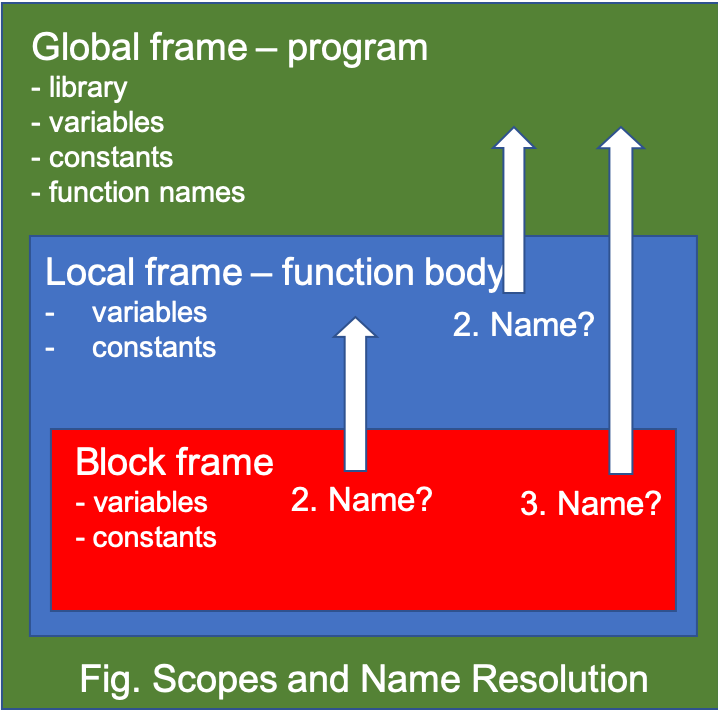
\includegraphics{resources/scopesandnameresolution.png}

    \hypertarget{visualize-identifiers-scopes-on-pythontutor.com}{%
\subsubsection{\texorpdfstring{visualize identifiers' scopes on
\href{http://pythontutor.com/cpp.html\#code=//\%20program\%20to\%20demonstrate\%20variable\%20scope\%0A//\%20libraries\%20have\%20global\%20scope\%0A\%23include\%20\%3Ciostream\%3E\%0A\%23include\%20\%3Cstring\%3E\%0A\%0Ausing\%20namespace\%20std\%3B\%0A\%0A//\%20global\%20identifiers\%0Aint\%20global_var\%20\%3D\%2010\%3B\%0Aconst\%20double\%20PI\%20\%3D\%203.141592653589793238\%3B\%0A\%23define\%20LF\%20'\%5Cn'\%0A\%0Aint\%20area_of_circle\%28const\%20float\%20radius\%29\%20\%7B\%0A\%20\%20global_var\%20\%3D\%20200\%3B\%0A\%20\%20return\%202*PI*radius\%3B\%0A\%7D\%0A\%0Aint\%20main\%28\%29\%20\%7B\%0A\%20\%20float\%20rad\%20\%3D\%202.5\%3B\%0A\%20\%20global_var\%20\%3D\%20100\%3B\%0A\%20\%20cout\%20\%3C\%3C\%20\%22area\%20of\%20circle\%20\%3D\%20\%22\%20\%3C\%3C\%20area_of_circle\%28rad\%29\%20\%3C\%3C\%20LF\%3B\%0A\%20\%20cout\%20\%3C\%3C\%20\%22global\%20var\%20\%3D\%20\%22\%20\%3C\%3C\%20global_var\%20\%3C\%3C\%20LF\%3B\%0A\%20\%20\%7B\%0A\%20\%20\%20\%20char\%20block_var\%20\%3D\%20'A'\%3B\%0A\%20\%20\%20\%20cout\%20\%3C\%3C\%20\%22block_var\%20within\%20block\%20\%3D\%20\%22\%20\%3C\%3C\%20block_var\%20\%3C\%3C\%20LF\%3B\%0A\%20\%20\%20\%20rad\%20\%3D\%2010.99f\%3B\%0A\%20\%20\%7D\%0A\%20\%20//\%20trying\%20to\%20access\%20block\%20variable\%20outside\%20block\%0A\%20\%20//\%20TODO\%3A\%20uncomment\%20the\%20following\%20and\%20compile\%0A\%20\%20//\%20block_var\%20\%3D\%20'a'\%3B\%0A\%20\%20return\%200\%3B\%0A\%7D\&curInstr=0\&mode=display\&origin=opt-frontend.js\&py=cpp\&rawInputLstJSON=\%5B\%5D}{pythontutor.com}}{visualize identifiers' scopes on pythontutor.com}}\label{visualize-identifiers-scopes-on-pythontutor.com}}

    \hypertarget{labs}{%
\subsection{Labs}\label{labs}}

\begin{enumerate}
\def\labelenumi{\arabic{enumi}.}
\tightlist
\item
  Write a C++ program that prompts the user to enter two points on a 2D
  geometry and finds the distance between the two points.

  \begin{itemize}
  \tightlist
  \item
    Use the partial solution provide in \texttt{pointDistance.cpp} file
    in \url{labs/functions/}
  \item
    Fix all the FIXMEs and write FIXED when each FIXME is fixed
  \end{itemize}
\end{enumerate}

    \hypertarget{exercises}{%
\subsection{Exercises}\label{exercises}}

\begin{enumerate}
\def\labelenumi{\arabic{enumi}.}
\tightlist
\item
  Write a C++ program including algorithm steps that calculates area and
  circumference of a circle.

  \begin{itemize}
  \tightlist
  \item
    must write functions to compute area and perimeter and automatically
    test each function with atleast 3 test cases
  \end{itemize}
\item
  Write a C++ program including algorithm steps that calculates Body
  Mass Index (BMI) of a person.

  \begin{itemize}
  \tightlist
  \item
    must use as many functions as possible
  \item
    write at least 3 test cases for each function
  \item
    more info on BMI -
    https://www.nhlbi.nih.gov/health/educational/lose\_wt/BMI/bmicalc.htm
  \item
    Formula
    \href{https://www.cdc.gov/healthyweight/assessing/bmi/childrens_bmi/childrens_bmi_formula.html\#:~:text=The\%20formula\%20for\%20BMI\%20is,to\%20convert\%20this\%20to\%20meters.\&text=When\%20using\%20English\%20measurements\%2C\%20pounds\%20should\%20be\%20divided\%20by\%20inches\%20squared}{here}.
  \item
    a sample solution is provided at \url{exercises/functions/BMI}
  \end{itemize}
\item
  Write a C++ program including algorithm steps that calculates area and
  perimeter of a triangle given three sides.

  \begin{itemize}
  \tightlist
  \item
    must write and use separate functions to calculate area and
    perimeter
  \item
    write at least 3 test cases for each function
  \item
    Hint: use Heron's formula to find area with three sides.
  \end{itemize}
\item
  Write a C++ program that converts hours into seconds.

  \begin{itemize}
  \tightlist
  \item
    must write and use function(s) to computer answer(s)
  \item
    must write at least 3 test cases for each function
  \item
    e.g.~given 2 hours, program should print 7200 as answer.
  \end{itemize}
\item
  Write a C++ program that converts seconds into hours, minutes and
  seconds.

  \begin{itemize}
  \tightlist
  \item
    must define and use function(s)
  \item
    write at least 3 test cases for each function
  \item
    sample input: 3600 sample output: 1 hour, 0 minute and 0 second
  \item
    sample input: 3661 sample output: 1 hour, 1 minute and 1 second
  \item
    Hint: use series of division and modulo operations
  \end{itemize}
\item
  Write a C++ program that finds area and perimeter of a rectangle.

  \begin{itemize}
  \tightlist
  \item
    must define and use function(s)
  \item
    write at least 3 test cases for each function
  \item
    a sample solution is provided her \url{demos/functions/rectangle}
  \end{itemize}
\end{enumerate}

\hypertarget{kattis-problems}{%
\subsection{Kattis Problems}\label{kattis-problems}}

\begin{itemize}
\tightlist
\item
  functions are not required to solve Kattis problems
\item
  however, it's best practices to use function to learn to be able to
  sovle harder and bigger problems
\end{itemize}

\begin{enumerate}
\def\labelenumi{\arabic{enumi}.}
\tightlist
\item
  Hello World! - https://open.kattis.com/problems/hello

  \begin{itemize}
  \tightlist
  \item
    solve the problem using function(s)
  \item
    write a test case for the function using assert
  \end{itemize}
\item
  Solving for Carrots - https://open.kattis.com/problems/carrots

  \begin{itemize}
  \tightlist
  \item
    solve the problem using function(s)
  \item
    using assert write at least three test cases for each function
  \end{itemize}
\item
  R2 - https://open.kattis.com/problems/r2

  \begin{itemize}
  \tightlist
  \item
    solve the problem using function(s)
  \item
    using assert write at least three test cases for each function
  \end{itemize}
\item
  Spavanac - https://open.kattis.com/problems/spavanac

  \begin{itemize}
  \tightlist
  \item
    solve the problem using function(s)
  \item
    using assert write at least three test cases for each function
  \end{itemize}
\item
  Add Two Numbers - https://open.kattis.com/problems/addtwonumbers

  \begin{itemize}
  \tightlist
  \item
    solve the problem using function(s)
  \item
    using assert write at least three test cases for each function
  \end{itemize}
\item
  Solve rest of the problems from Chapter 3 - Std IO using as many
  functions as possible.

  \begin{itemize}
  \tightlist
  \item
    using assert write at least three test cases for each function
  \end{itemize}
\end{enumerate}

    \hypertarget{summary}{%
\subsection{Summary}\label{summary}}

\begin{itemize}
\tightlist
\item
  this chapter covered concepts on functions; how to create new
  functions and use them
\item
  went over various types of functions (fruitful and fruitless)
\item
  learned about why and how to pass data to functions
\item
  learned about debugging using assert(), cerr (stderr stream)
\item
  learned about important foundation concept of automatically testing
  functions
\item
  covered function overloading and templating
\item
  finally, exercises and sample solutions
\end{itemize}

    \begin{tcolorbox}[breakable, size=fbox, boxrule=1pt, pad at break*=1mm,colback=cellbackground, colframe=cellborder]
\prompt{In}{incolor}{ }{\boxspacing}
\begin{Verbatim}[commandchars=\\\{\}]

\end{Verbatim}
\end{tcolorbox}


    % Add a bibliography block to the postdoc
    
    
    
\end{document}
